\documentclass[fontset = none, t]{ctexbeamer}

% 载入需要的宏包
% 加载宏包
%===================注意======================%
% 在调用beamer.cls宏包后,以下宏包将自动调用,
% 不应单独调用这些宏包,以免发生冲突
% amsfonts, amsmath, amssymb, amsthm, 
% enumerate, geometry, graphics, graphicx, 
% hyperref, url, 
% ifpdf, keyval, xcolor, xxcolor
% =============================================%
% % 调整行间距
\usepackage{setspace}

\usepackage{fontawesome5}

\usepackage{unicode-math}

\usepackage{qrcode}

\usepackage{multicol}

\usepackage{csquotes}

% ========排版键盘组合和菜单的宏包=========
\usepackage{menukeys}

% 代码排版工具宏包
% 需要预先安装 python 和 pygments。
% 此宏包要加  -shell-escape 编译参数
% 版本2.0,支持行内代码排版
\usepackage{minted}

% 特殊符号
\usepackage{pifont}

%%% Local Variables: 
%%% mode: latex
%%% TeX-master: "../main.tex"
%%% End:


% 进行必要的设置
\makeatletter
% pretend to already have loaded beamerfontthememetropolis
\@namedef{ver@beamerfontthememetropolis.sty}{9999/99/99}

% Beamer theme
\usetheme{Xiaoshan}

% 设置字体(参考曾祥东的latex-talk.tex进行设置)
%\usefonttheme{serif,professionalfonts}
\usefonttheme{professionalfonts}
% 加载字体
\setmainfont{LibertinusSerif}[% 英文字体
  Extension      = .otf,
  UprightFont    = *-Regular,
  BoldFont       = *-Bold,
  ItalicFont     = *-Italic,
  BoldItalicFont = *-BoldItalic,
  Scale          = 1.0]
\setmonofont{Iosevka}[Scale=1.0]% 等宽字体,主要用于代码排版
\setmathfont{LibertinusMath-Regular.otf}% Iosevka数学字体,需要unicode-math支持
\setCJKmainfont{Source Han Serif SC}[ % 中文衬线字体,思源宋体
  UprightFont     = * SemiBold,
  BoldFont        = * Heavy,
  ItalicFont      = * Light,
  BoldItalicFont  = * Medium,
  RawFeature      = +fwid]
\setCJKsansfont{Source Han Sans SC}[ % 中文无衬线字体,思源宋体
  UprightFont     = * Medium,
  BoldFont        = * Heavy,
  ItalicFont      = * Light,
  BoldItalicFont  = * Normal,
  RawFeature      = +fwid]  
\setCJKmonofont{Sarasa Mono SC}[% 中文等宽字体,Sarasa Mono SC
  UprightFont     = * Medium,
  BoldFont        = * Medium,
  ItalicFont      = * Extralight,
  BoldItalicFont  = * Light,
  RawFeature      = +fwid]   
% 中文衬线字体,思源字体,请将字体置于fonts目录下
% \setCJKmainfont[Extension=.otf,
%     Path=fonts/,
%     UprightFont=NotoSerifCJKsc-Regular,
%     BoldFont=NotoSerifCJKsc-Bold,
%     ItalicFont=NotoSerifCJKsc-Regular,
%     BoldItalicFont=NotoSerifCJKsc-Bold,
%     ItalicFeatures=FakeSlant,
%     BoldItalicFeatures=FakeSlant]{NotoSerifCJKsc}
% % 无衬线字体,思源字体,请将字体置于fonts目录下         
% \setCJKsansfont[
%     Extension=.otf,
%     Path=fonts/,
%     UprightFont=NotoSansCJKsc-Regular,
%     BoldFont=NotoSansCJKsc-Bold,
%     ItalicFont=NotoSansCJKsc-Regular,
%     BoldItalicFont=NotoSansCJKsc-Bold,
%     ItalicFeatures=FakeSlant,
%     BoldItalicFeatures=FakeSlant]{NotoSansSC}
% % 中文等宽字体,思源字体,请将字体置于fonts目录下  
% \setCJKmonofont[
%     Extension=.otf,
%     Path=fonts/,
%     UprightFont=NotoSansMonoCJKsc-Regular,
%     BoldFont=NotoSansMonoCJKsc-Bold,
%     ItalicFont=NotoSansMonoCJKsc-Regular,
%     BoldItalicFont=NotoSansMonoCJKsc-Bold,
%     ItalicFeatures=FakeSlant,
%     BoldItalicFeatures=FakeSlant]{NotoSansMonoSC}

% Beamer settings
\metroset{progressbar=none}
\setbeamerfont{title}{size=\huge, series=\bfseries}
\setbeamerfont*{subtitle}{size=\large, shape=\itshape}
\setbeamerfont{section title}{size=\Large, series=\bfseries}
\setbeamerfont{frametitle}{size=\large, series=\bfseries}%family = \rmfamily, 
\setbeamerfont{caption}{size=\footnotesize, series=\bfseries}
\setbeamerfont{footnote}{size=\tiny}
\setbeamerfont{alerted text}{series=\bfseries}
\addtobeamertemplate{institute}{\raggedleft}{}
\setbeamertemplate{title}{%
  \raggedleft
  \linespread{1.0}%
  \inserttitle
  \hspace*{1.2cm}\par
  \vspace*{0.5em}}
\setbeamertemplate{subtitle}{%
  \raggedleft
  \insertsubtitle
  \hspace*{1.2cm}\par
  \vspace*{0.5em}}
\setbeamertemplate{title page}{
  \vfill
  \begin{minipage}[c]{\textwidth}    
    \usebeamertemplate*{title graphic}\vfill
    \usebeamertemplate*{title}
    \usebeamertemplate*{subtitle}
    \usebeamertemplate*{title separator}
    \usebeamertemplate*{author}
    \usebeamertemplate*{date}
    \usebeamertemplate*{institute}
    \vfill
  \end{minipage}}
\setbeamertemplate{frame numbering}{{\insertframenumber/\inserttotalframenumber}}%\zhnumber[style=Financial]
\setbeamertemplate{itemize/enumerate subbody begin}{\footnotesize}
\setbeamertemplate{caption}{\parbox{\textwidth}{\centering\insertcaption}\par}
\setbeamertemplate{bibliography item}[text]

% 设置帧标题格式
\setbeamertemplate{frametitle}{
    \ifbeamercolorempty[bg]{frametitle}{}{\nointerlineskip}%
    \@tempdima=\textwidth%
    \advance\@tempdima by\beamer@leftmargin%
    \advance\@tempdima by\beamer@rightmargin%
    %\hspace*{1cm} %%%%%%%%%%%%% For example insert shift to right
    \begin{beamercolorbox}[sep=0.3cm,wd=\the\@tempdima]{frametitle}
        \usebeamerfont{frametitle}%
        \vbox{}\vskip-1ex%
        \if@tempswa\else\csname beamer@ftecenter\endcsname\fi%
        \strut\insertframesubtitle\hfill\strut%\par%
        {%
            \ifx\insertframetitle\@empty%
            \else%
            {\usebeamerfont{frametitle}\usebeamercolor[fg]{frametitle}|\insertframetitle\strut}%\par}%
            \fi
        }%
        \vskip-1ex%
        \if@tempswa\else\vskip-.3cm\fi% set inside beamercolorbox... evil here...
    \end{beamercolorbox}%
  }

% 设置列表符号
\setbeamertemplate{itemize item}{\scriptsize\raise1.25pt\hbox{\donotcoloroutermaths \ding{42}}}%$\blacktriangleright$}}
\setbeamertemplate{itemize subitem}{\tiny\raise1.5pt\hbox{\donotcoloroutermaths \ding{43}}}%$\blacktriangleright$}}
\setbeamertemplate{itemize subsubitem}{\tiny\raise1.5pt\hbox{\donotcoloroutermaths \ding{45}}}%$\blacktriangleright$}}
\setbeamertemplate{enumerate item}{\insertenumlabel.}
\setbeamertemplate{enumerate subitem}{\insertenumlabel.\insertsubenumlabel}
\setbeamertemplate{enumerate subsubitem}{\insertenumlabel.\insertsubenumlabel.\insertsubsubenumlabel}
\setbeamertemplate{enumerate mini template}{\insertenumlabel}  
  
% 设置页脚
\setbeamertemplate{footline}
{
    \leavevmode%
    \hbox{%
        \begin{beamercolorbox}[wd=.25\paperwidth,ht=2.25ex,dp=1ex,center]{frametitle}%{author in head/foot}%
            \usebeamerfont{author in head/foot}\insertauthor{}(\insertshortauthor{})
        \end{beamercolorbox}%
        \begin{beamercolorbox}[wd=.5\paperwidth,ht=2.25ex,dp=1ex,center]{frametitle}%{title in head/foot}%
            \usebeamerfont{title in head/foot}\insertshorttitle
        \end{beamercolorbox}%
        \begin{beamercolorbox}[wd=.25\paperwidth,ht=2.25ex,dp=1ex,right]{frametitle}%{date in head/foot}%
            \usebeamerfont{date in head/foot}\insertshortinstitute{}\hspace*{2em}
            \insertframenumber{}/\inserttotalframenumber{}\hspace*{2ex} 
        \end{beamercolorbox}}%
        \vskip0pt%
    }

%改变脚注的符号
\setbeamerfont{footnote}{size=\zihao{7}} % 改变脚注字号
\makeatletter
\def\@fnsymbol#1{\ensuremath{\ifcase#1\or *\or \dagger\or \ddagger\or
   \mathsection\or \mathparagraph\or \|\or **\or \dagger\dagger
   \or \ddagger\ddagger \else\@ctrerr\fi}}
\makeatother
\renewcommand{\thefootnote}{\fnsymbol{footnote}}

\DeclareRobustCommand{\nonumberfootnote}[2][]{%
  \let\thefootnote\relax
  \footnotetext#1{#2}}    

\makeatletter
\def\@fnsymbol#1{\ensuremath{\ifcase#1\or *\or \dagger\or \ddagger\or
   \mathsection\or \mathparagraph\or \|\or **\or \dagger\dagger
   \or \ddagger\ddagger \else\@ctrerr\fi}}
\renewcommand{\thefootnote}{\fnsymbol{footnote}}
\makeatother

% PoZheHao, see https://github.com/CTeX-org/ctex-kit/issues/382
\ExplSyntaxOn
\xeCJK_new_class:n { PoZheHao }
\__xeCJK_save_CJK_class:n { PoZheHao }
\xeCJK_declare_char_class:nn { PoZheHao } { "2014 }
\seq_map_inline:Nn \g__xeCJK_class_seq
  {
    \str_if_eq:nnF {#1} { PoZheHao }
      {
        \xeCJK_copy_inter_class_toks:nnnn { PoZheHao } {#1} { FullRight } {#1}
        \xeCJK_copy_inter_class_toks:nnnn {#1} { PoZheHao } {#1} { FullRight }
      }
  }
\ExplSyntaxOff


%% 自定义相关的名称宏命令
%% ==================================================
%% \newcommand{\yourcommand}[参数个数]{内容}
% 西北农林科技大学各单位名称
\newcommand{\nwsuaf}{西北农林科技大学}
\newcommand{\cie}{信息工程学院}
\newcommand{\cs}{计算机科学系}


%% 签署春秋学期日期命令
\newcommand{\tomonth}{
  \the\year 年\the\month 月
}


\newcommand{\tomonthen}{
  \ifcase\the\month
  \or January%
  \or February%
  \or March%
  \or April%
  \or May%
  \or June%
  \or July%
  \or August%
  \or September%
  \or October%
  \or November%
  \or December%
  \fi, \the\year
}

\newcommand{\tosemester}{
  \the\year 年\ 
  \ifcase\the\month
  \or 秋%
  \or 春%
  \or 春%
  \or 春%
  \or 春%
  \or 春%
  \or 春%
  \or 夏%
  \or 秋%
  \or 秋%
  \or 秋%
  \or 秋%
  \fi 
}

\newcommand{\tosemesteren}{  
  \ifcase\the\month
  \or Autumn%
  \or Spring%
  \or Spring%
  \or Spring%
  \or Spring%
  \or Spring%
  \or Summer%
  \or Autumn%
  \or Autumn%
  \or Autumn%
  \or Autumn%
  \or Autumn%
  \fi, \the\year
}

%%%%%%%%%%%%%%%%%%%%%%%%%%%%%%%%%%%%%%%%%%%%%%%%%%%%%%%%%%%%%%%%%%%%%%
% LaTeX Overlay Generator - Annotated Figures v0.0.2
% Created with http://ff.cx/latex-overlay-generator/
% If this generator saves you time, consider donating 5,- EUR! :-)
%%%%%%%%%%%%%%%%%%%%%%%%%%%%%%%%%%%%%%%%%%%%%%%%%%%%%%%%%%%%%%%%%%%%%%
%                         #1          #2       #3         #4           #5          #6            #7           #8
%\annotatedFigureBox{bottom-left}{top-right}{label}{label-position}{box-color}{label-color}{border-color}{text-color}
\newcommand*\annotatedFigureBoxCustom[8]{\draw[#5,thick,rounded corners] (#1) rectangle (#2);\node at (#4) [fill=#6,thick,shape=circle,draw=#7,inner sep=2pt,font=\sffamily,text=#8] {\textbf{#3}};}
\newcommand*\annotatedFigureBoxLabel[4]{\annotatedFigureBoxCustom{#1}{#2}{#3}{#4}{red}{white}{black}{black}}
\newcommand*\annotatedFigureBox[3]{\draw[#3,thick,rounded corners=0.5mm] (#1) rectangle (#2);}
\newenvironment {annotatedFigure}[1]{\centering\begin{tikzpicture}\node[anchor=south west,inner sep=0] (image) at (0,0) { #1};\begin{scope}[x={(image.south east)},y={(image.north west)}]}{\end{scope}\end{tikzpicture}}
%%%%%%%%%%%%%%%%%%%%%%%%%%%%%%%%%%%%%%%%%%%%%%%%%%%%%%%%%%%%%%%%%%%%%%

\newcommand\CASE[1]{{\addfontfeatures{Letters=Uppercase}#1}}
\newcommand\jatext[1]{{\addCJKfontfeatures{Language=Japanese}#1}}
% 超链接及符号
\newcommand\link[1]{\href{#1}{\ \faExternalLinkSquare*}}


% % 定义TeXLive的LOGO
\definecolor{tlblue}{HTML}{0078B8}
\newcommand*\TeXLive{T\kern -.1667em\lower .5ex\hbox {E}\kern
  -.025emX\,Live}
\newcommand\tl[1][2019]{\TeXLive ~ #1}
\newcommand\tlive[1][2019]{
  \begin{tikzpicture}[x=1pt,y=1pt,inner sep=0pt,outer sep=0pt]
    \fill [tlblue] (0,0) rectangle (567,160);
    \node [white] at (29.7,33.8) [anchor=south west]
    {\scalebox{10}{\bfseries\TeXLive\~ #1}};
    \node at (388,9) [anchor=south west] {
\includegraphics[width=15em]{tl-lion}};
    % \node [anchor=south west] {
\includegraphics[height=16em]{logo}};
  \end{tikzpicture}%
}

% 动态改变menukeys宏包的win/mac样式
\makeatletter
\def\setmenukeyswin{\def\tw@mk@os{win}}
\def\setmenukeysmac{\def\tw@mk@os{mac}}
\makeatother

% 设置minted宏包编排代码的参数及用于latex代码排版的简化命令
\setminted{fontsize=\footnotesize, breaklines=true, breakautoindent=false}
\newmintinline{tex}{fontsize=\footnotesize}
\newmintinline{sh}{breaklines=true}
\newmintinline[texinlinett]{tex}{escapeinside=||}
\newminted{tex}{fontsize=\scriptsize, bgcolor=yellow!20, frame=lines, autogobble}
\newminted[texcodett]{tex}{autogobble, fontsize=\scriptsize, bgcolor=yellow!20, frame=lines, escapeinside=||}
\newminted[shell]{sh}{autogobble,frame=lines}
\newmintedfile{tex}{bgcolor=yellow!20, fontsize=\footnotesize, frame=lines}

% 插图路径设置
% ==================================================
\graphicspath{{figures/}}%图片所在的目录
% ==================================================

%%% Local Variables: 
%%% mode: latex
%%% TeX-master: "../main.tex"
%%% End: 


% Information
\title[\TeXLive 的安装]{\TeXLive 的安装简单教程}
\author[N. Geng]{耿楠}
\institute[教发中心]{西北农林科技大学教学发展中心}
\date{\tosemester}
\titlegraphic{%
  \vspace{3.0cm}
  \qrcode[hyperlink, height=1.6cm]{https://github.com/registor/install-texlive-studio}}

\begin{document}

\maketitle

\section[下载\TeXLive]{下载\TeXLive 镜像文件}
\begin{frame}{下载\TeXLive}{ISO镜像文件}
  \begin{itemize}
  \item 下载
    \begin{itemize}
    \item http://www.tug.org/texlive/\link{http://www.tug.org/texlive/}
      \begin{itemize}
      \item 单击\alert{\tl}下载链接
      \end{itemize}
    \end{itemize}
  \end{itemize}  
  \centering
  %\vfill
  %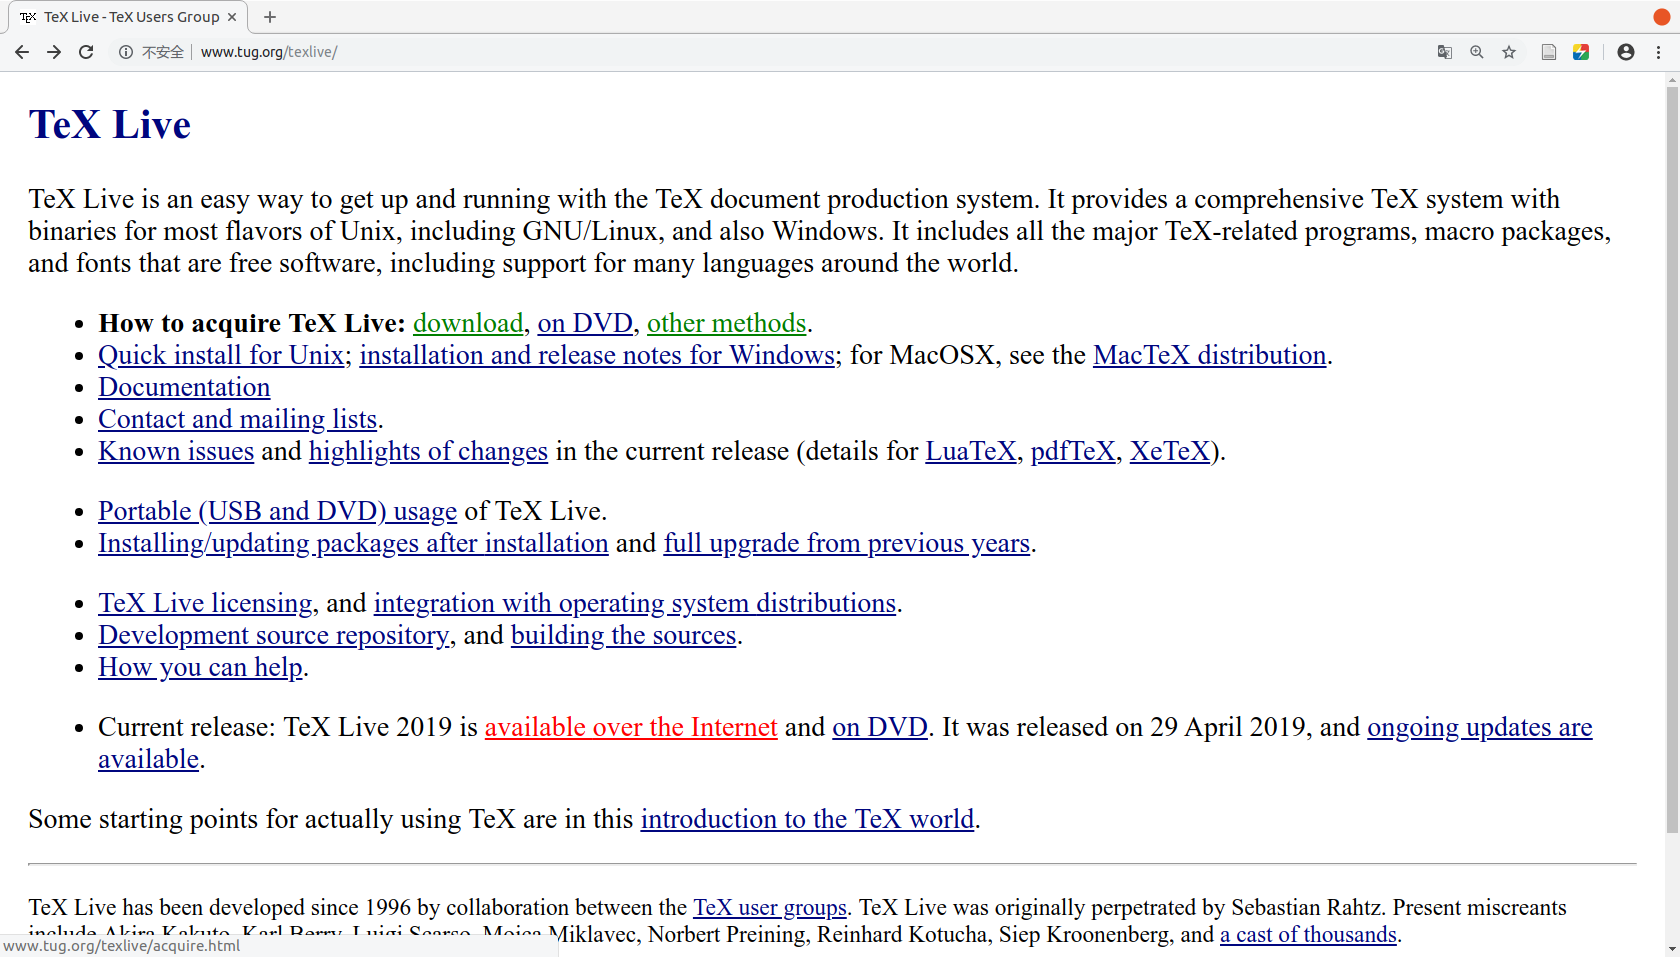
\includegraphics[width=0.48\textwidth]{downloadiso/tugtexlive}\quad
  %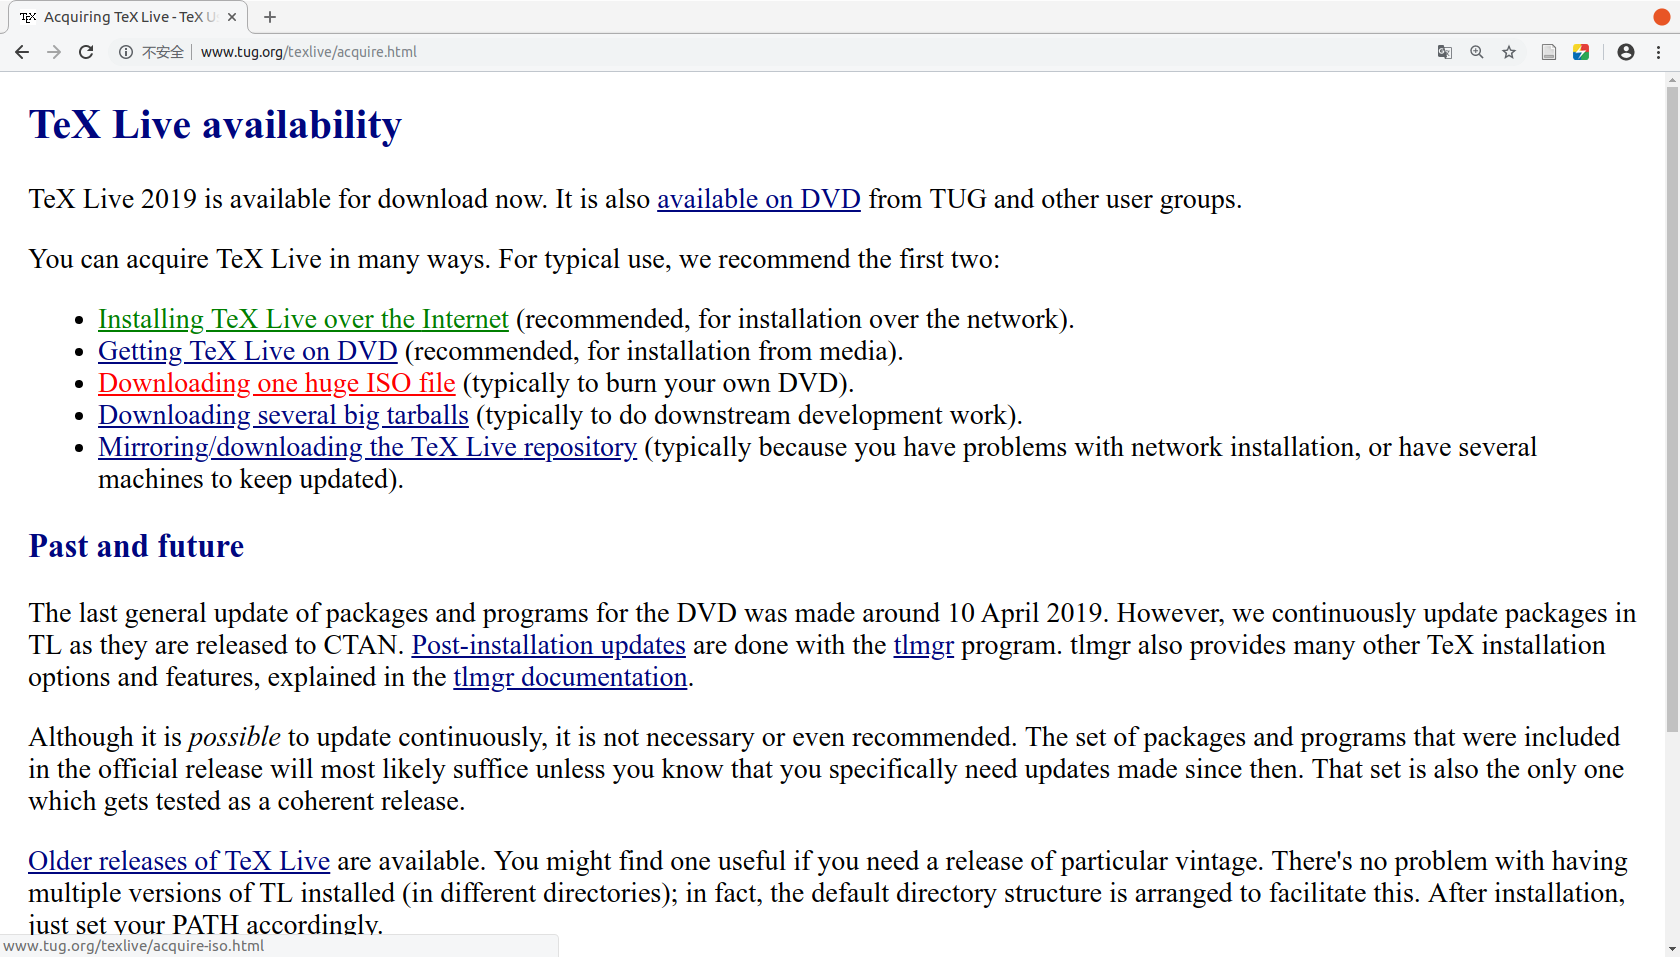
\includegraphics[width=0.48\textwidth]{downloadiso/downloadlink}
  % \vfill
  \begin{annotatedFigure}
    {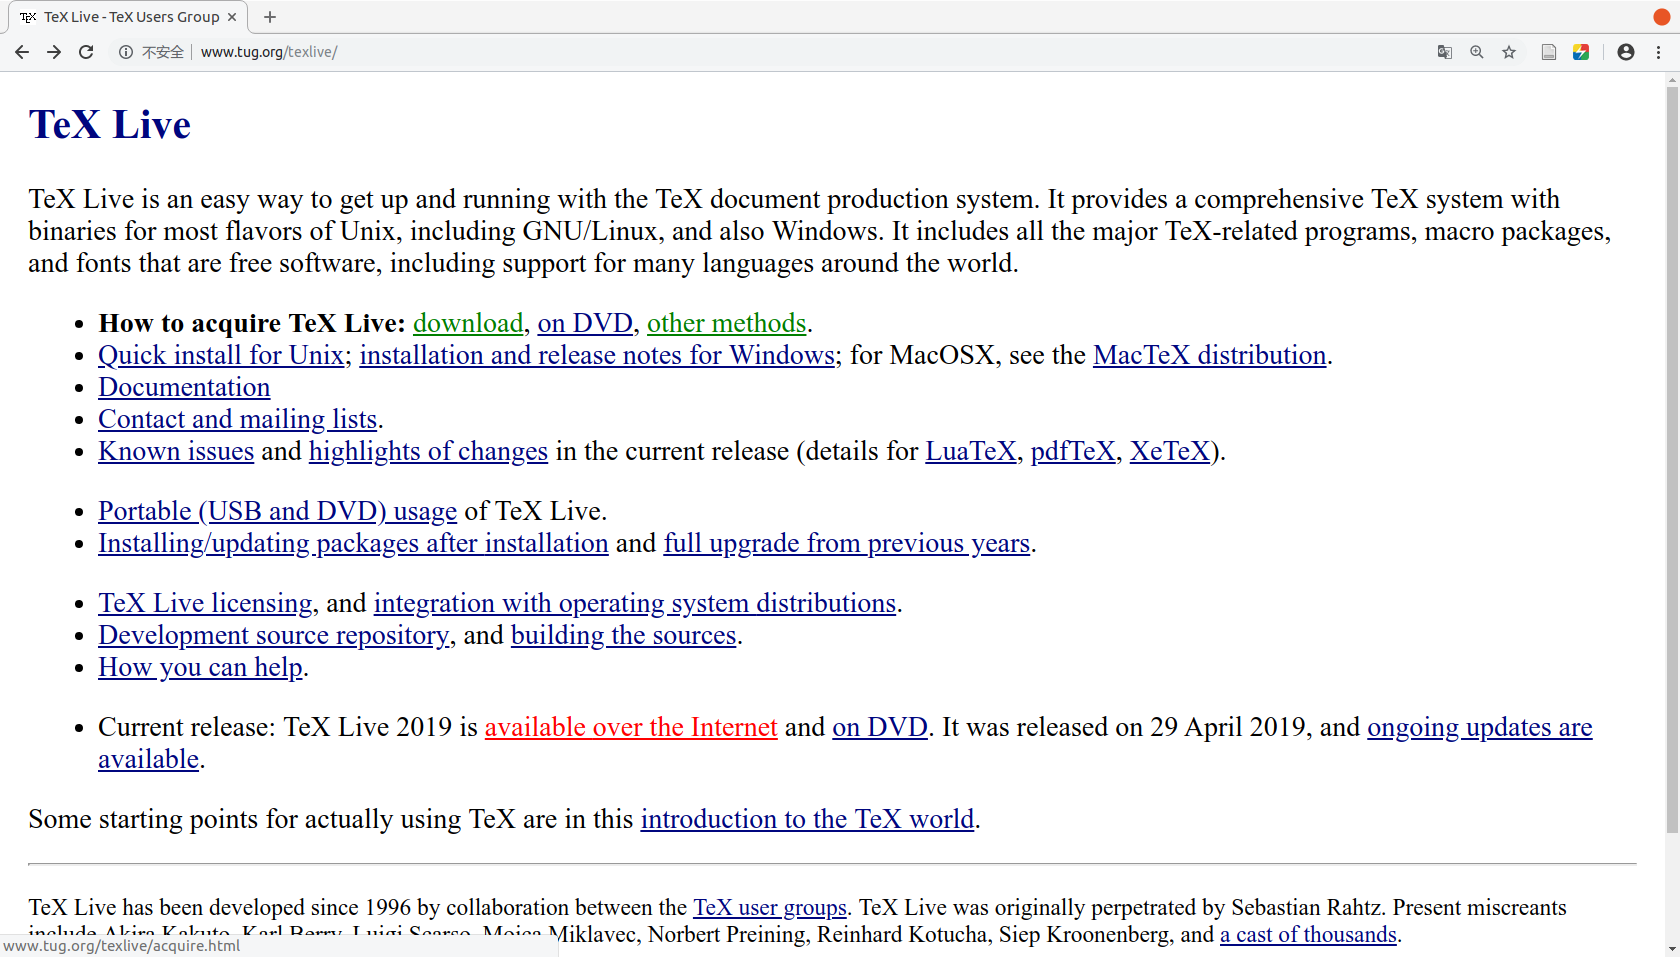
\includegraphics[width=0.9\textwidth]{downloadiso/tugtexlive}}
    \annotatedFigureBox{0.281,0.216}{0.47,0.26}{blue}
  \end{annotatedFigure}
\end{frame}

\begin{frame}{下载\TeXLive}{ISO镜像文件}
  \begin{itemize}
  \item 下载
    \begin{itemize}
    \item http://www.tug.org/texlive/\link{http://www.tug.org/texlive/}
      \begin{itemize}
      \item 单击\alert{ISO镜像文件}下载链接
      \end{itemize}
    \end{itemize}
  \end{itemize}  
  \centering
  %\vfill
  %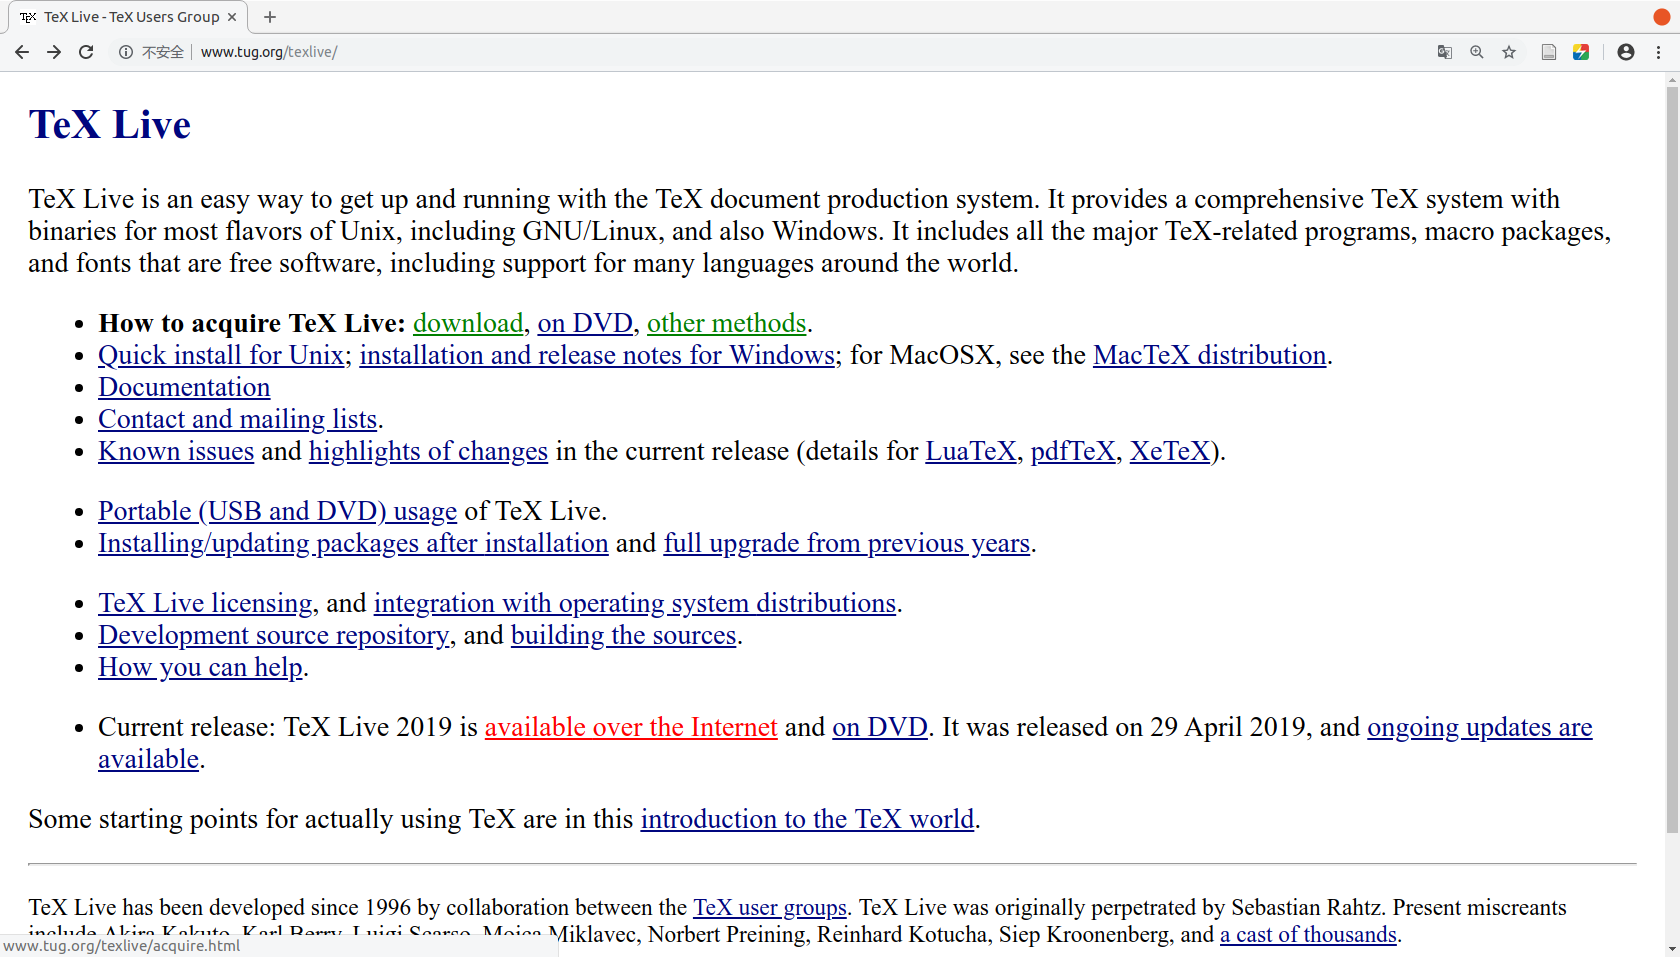
\includegraphics[width=0.48\textwidth]{downloadiso/tugtexlive}\quad
  %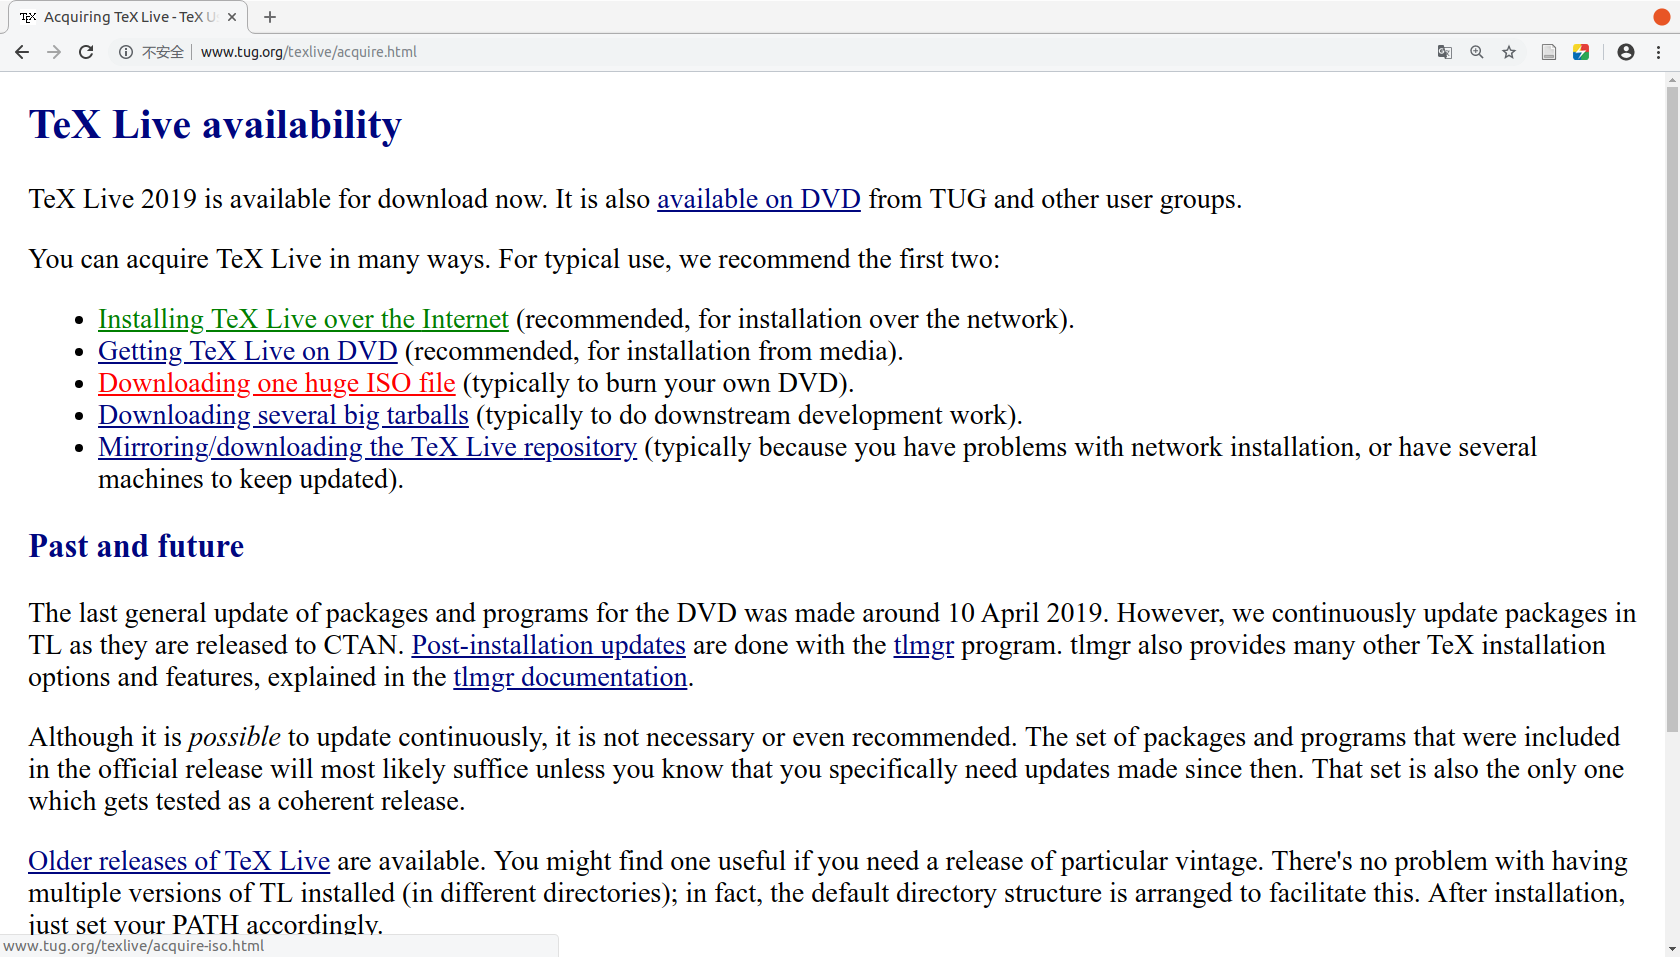
\includegraphics[width=0.48\textwidth]{downloadiso/downloadlink}
  % \vfill
  \begin{annotatedFigure}
    {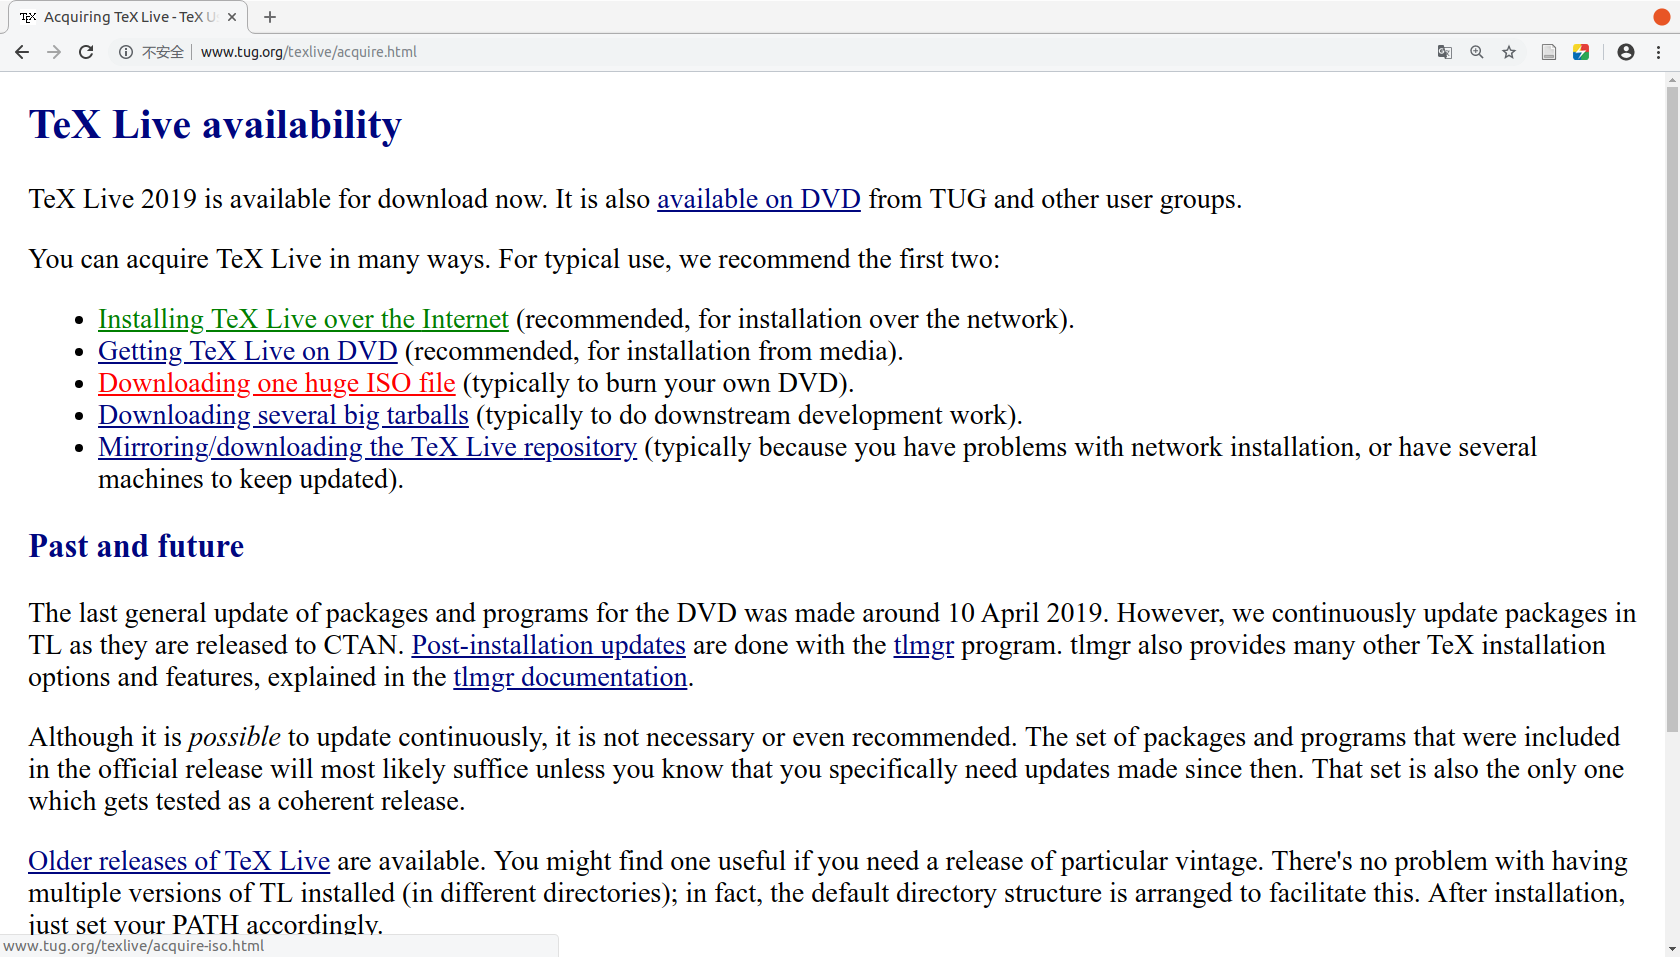
\includegraphics[width=0.9\textwidth]{downloadiso/downloadlink}}
    \annotatedFigureBox{0.04,0.577}{0.285,0.62}{blue}
  \end{annotatedFigure}
\end{frame}

\begin{frame}{下载\TeXLive}{ISO镜像文件}  
  \begin{itemize}
  \item 下载
    \begin{itemize}
    \item http://www.tug.org/texlive/\link{http://www.tug.org/texlive/}
      \begin{itemize}
      \item 自动选择\alert{镜像网站}
      \end{itemize}
    \end{itemize}
  \end{itemize}
  \centering
  % \vfill
  % 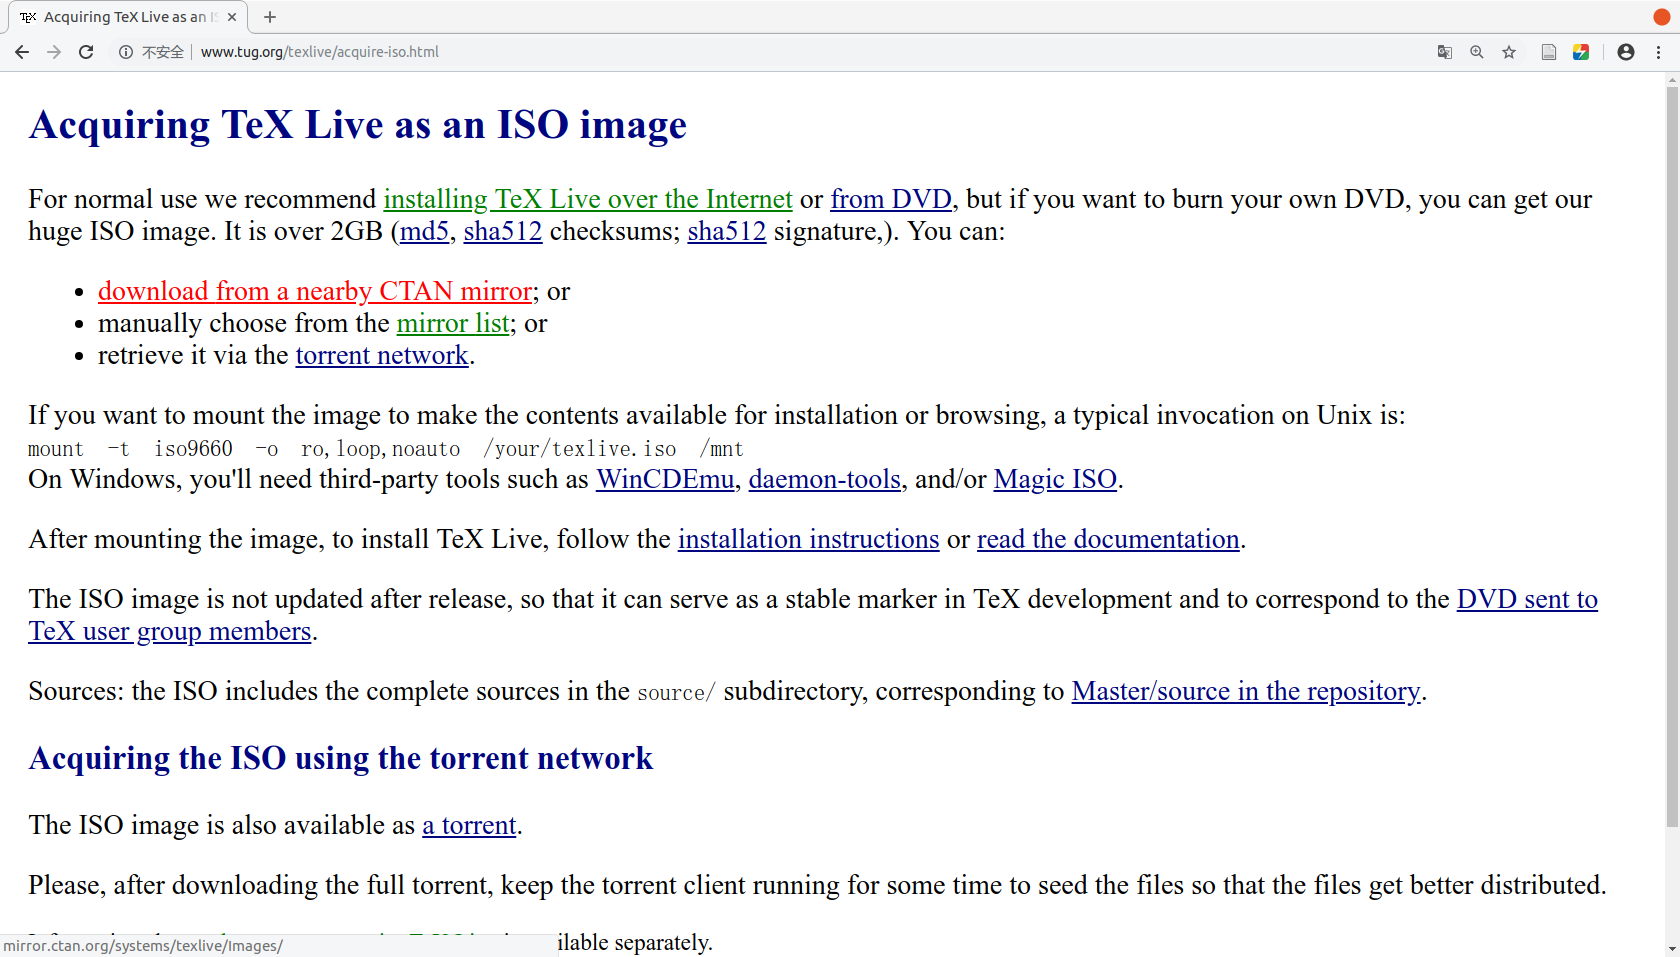
\includegraphics[width=0.48\textwidth]{downloadiso/mirrolink}\quad
  % 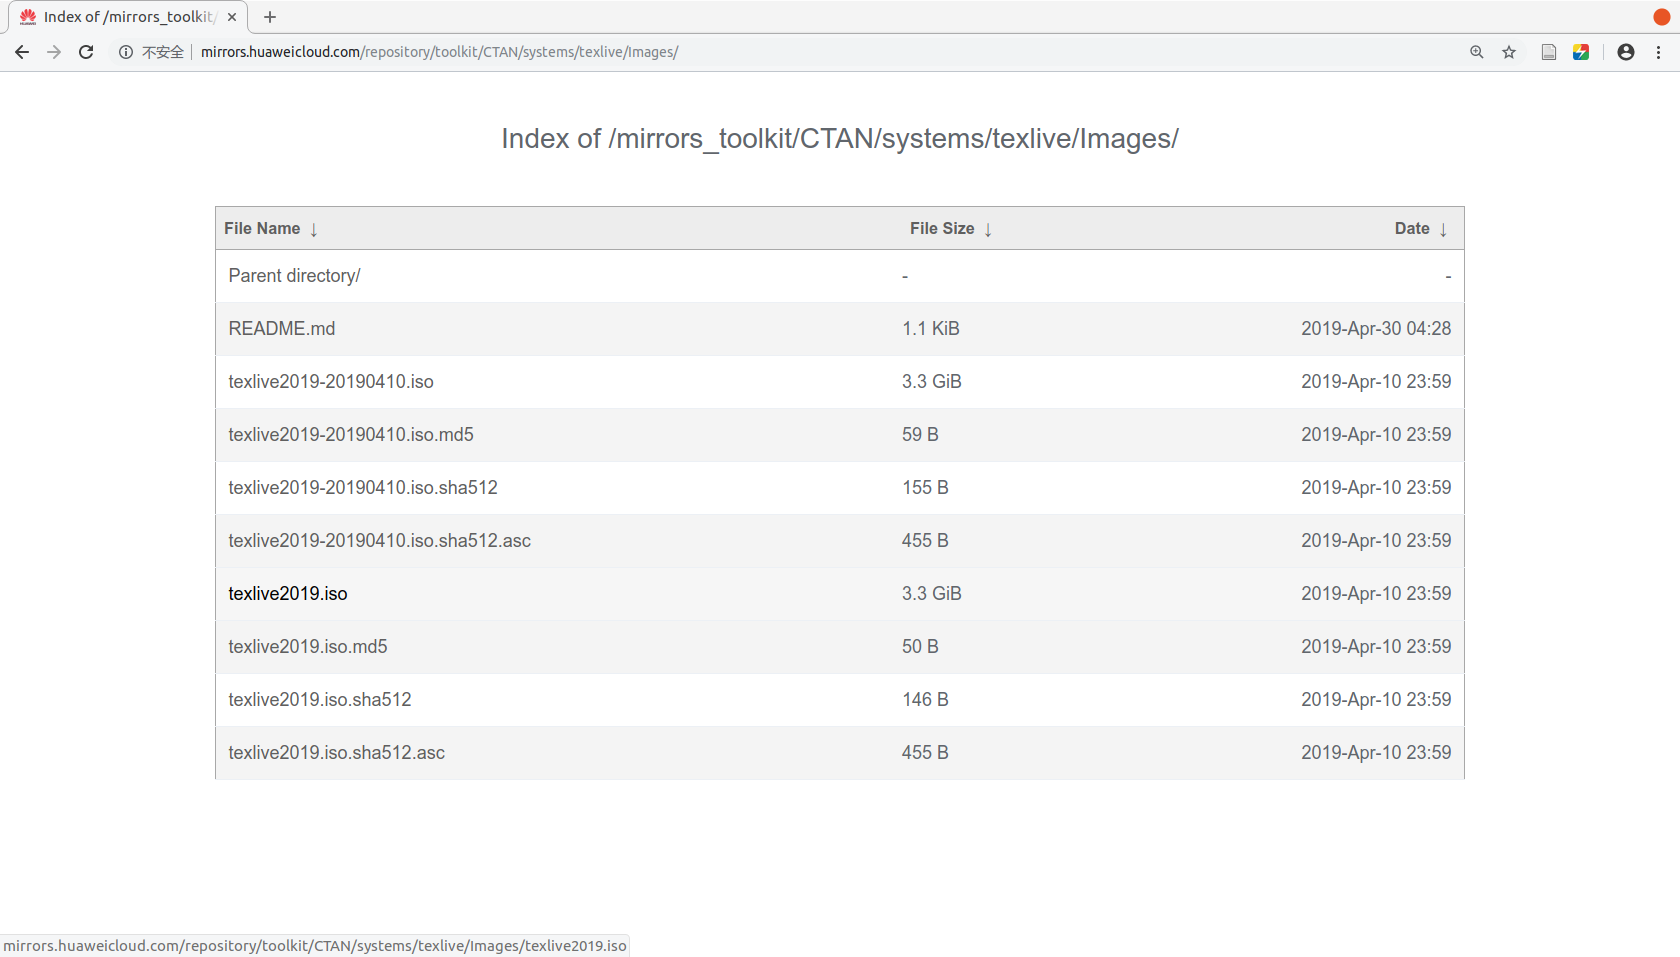
\includegraphics[width=0.48\textwidth]{downloadiso/isofilelist}
  % \vfill
  \begin{annotatedFigure}
    {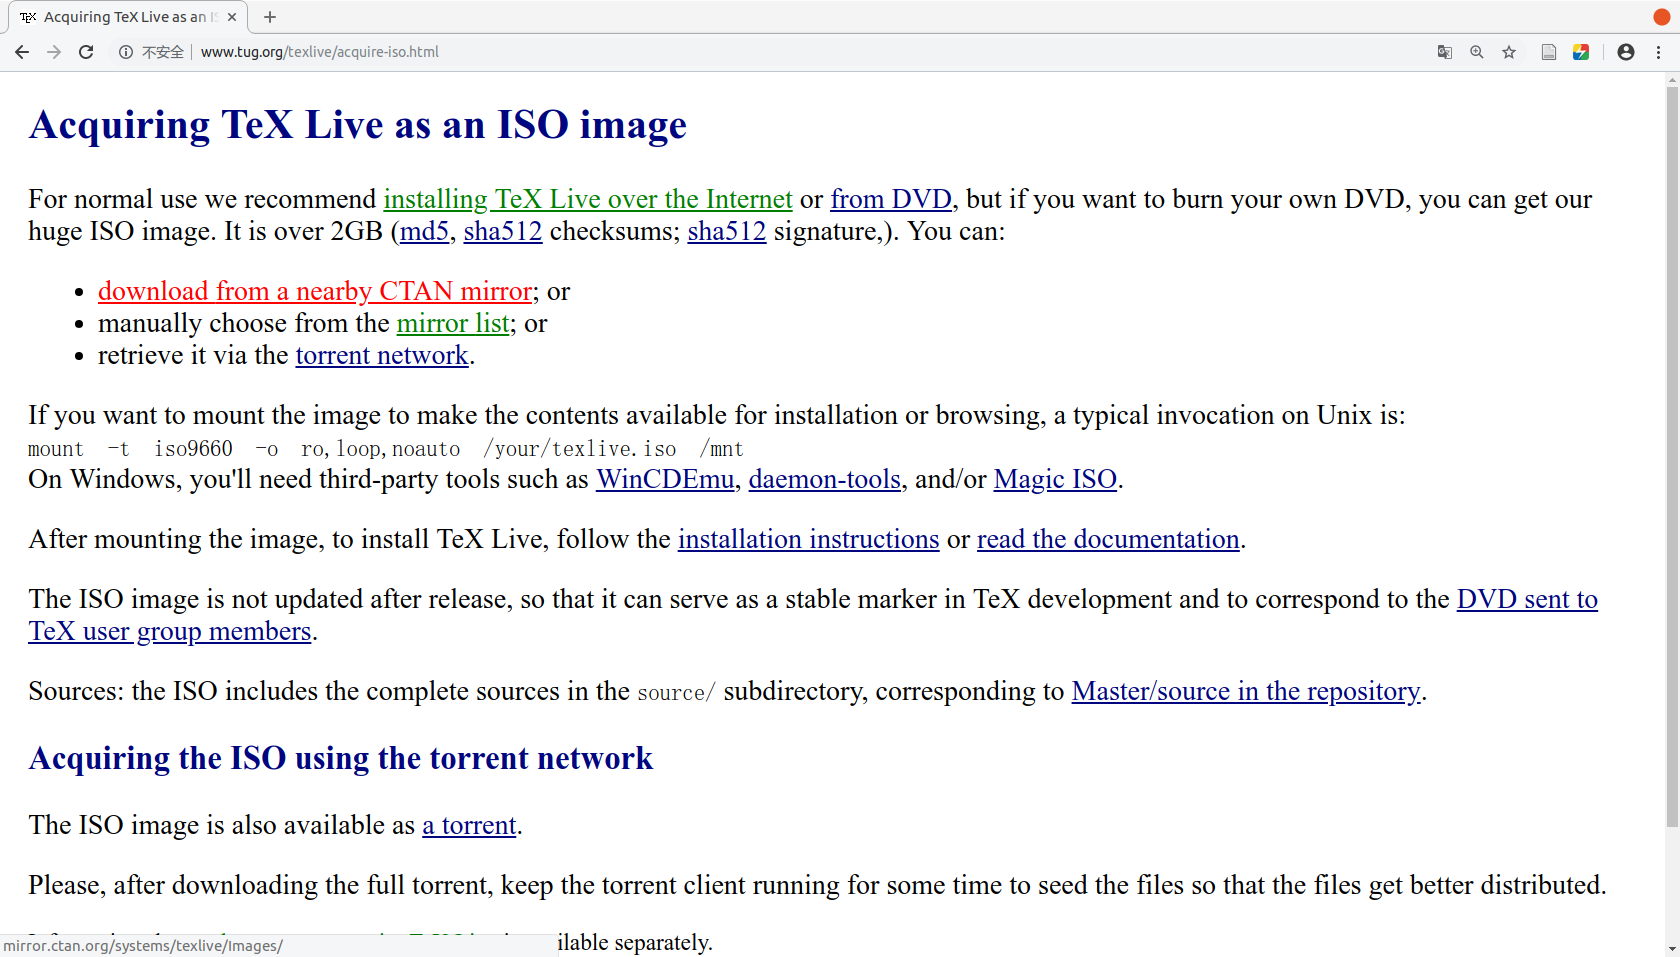
\includegraphics[width=0.9\textwidth]{downloadiso/mirrolink}}
    \annotatedFigureBox{0.04,0.674}{0.326,0.715}{blue}
  \end{annotatedFigure}
\end{frame}

\begin{frame}{下载\TeXLive}{ISO镜像文件}  
  \begin{itemize}
  \item 下载
    \begin{itemize}
    \item http://www.tug.org/texlive/\link{http://www.tug.org/texlive/}
      \begin{itemize}
      \item 任选1个下载(\alert{3.3GiB})
      \end{itemize}
    \end{itemize}    
  \end{itemize}
  \centering
  % \vfill
  % 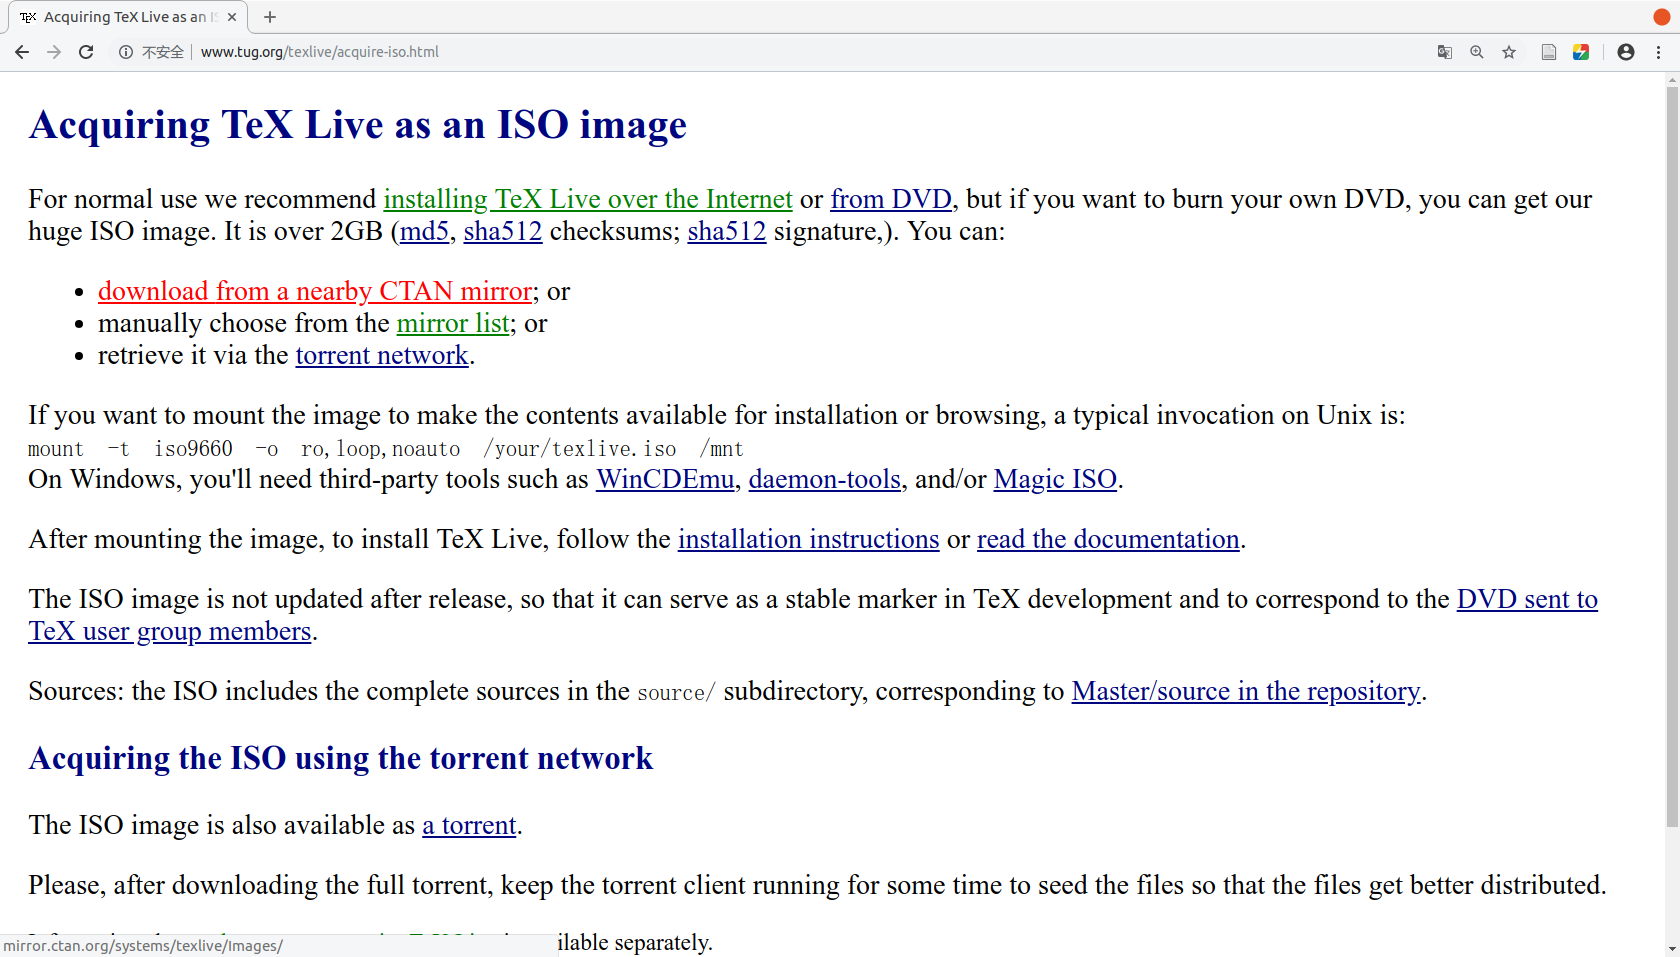
\includegraphics[width=0.48\textwidth]{downloadiso/mirrolink}\quad
  % 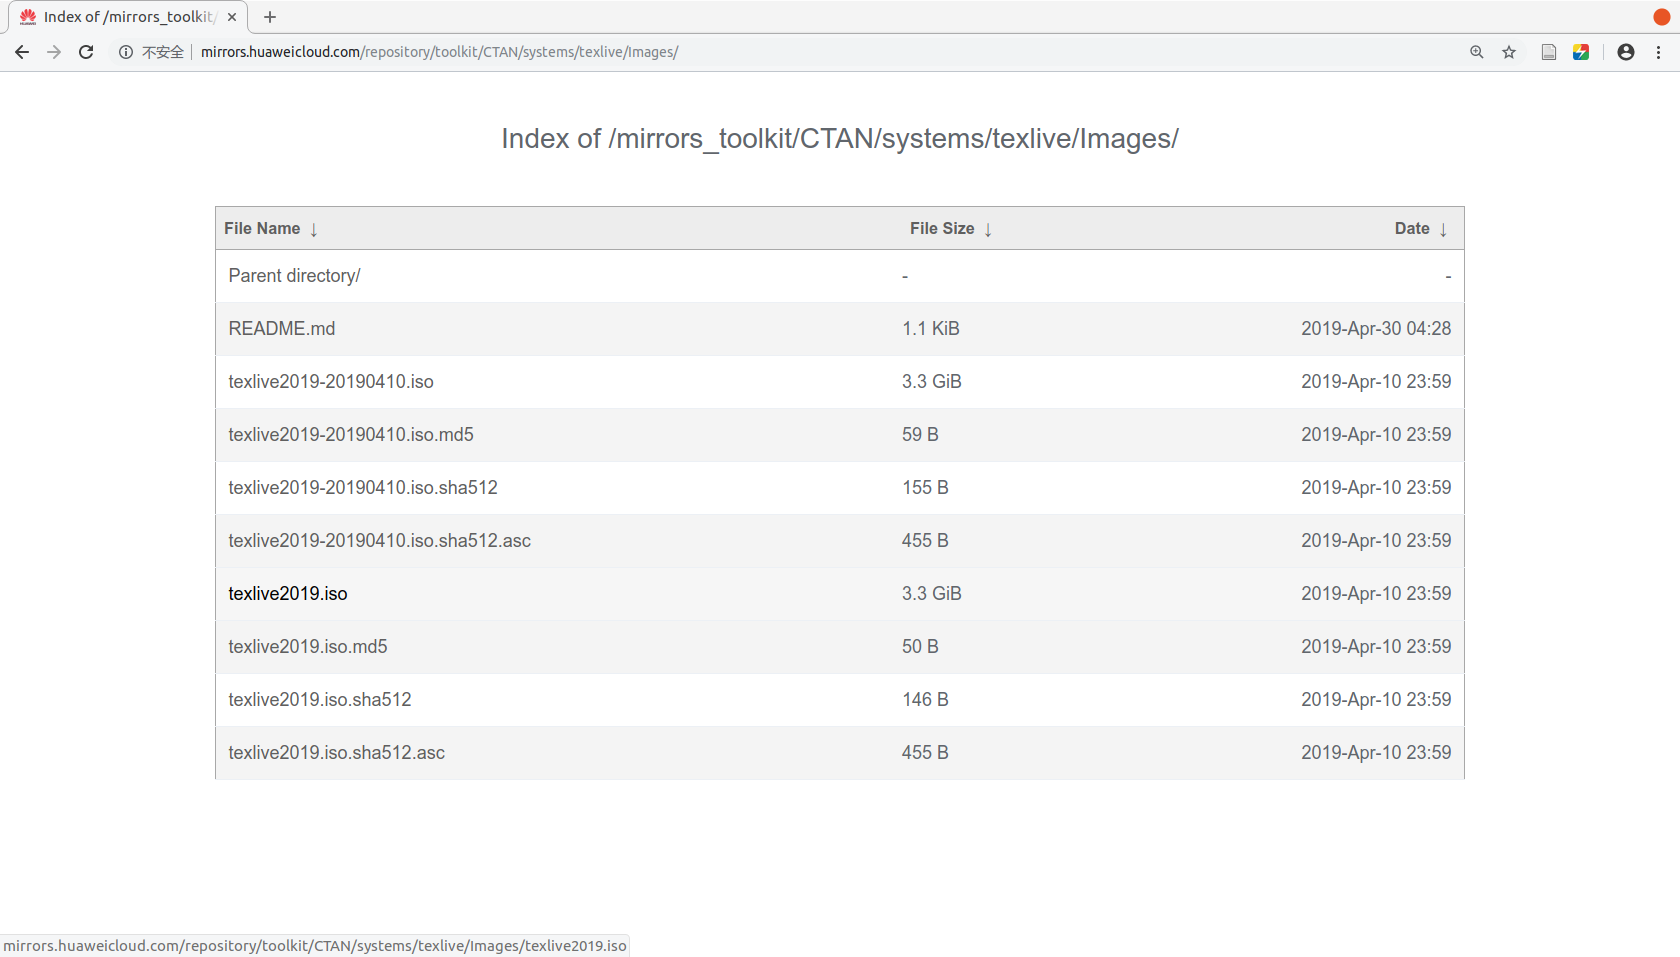
\includegraphics[width=0.48\textwidth]{downloadiso/isofilelist}
  % \vfill
  \begin{annotatedFigure}
    {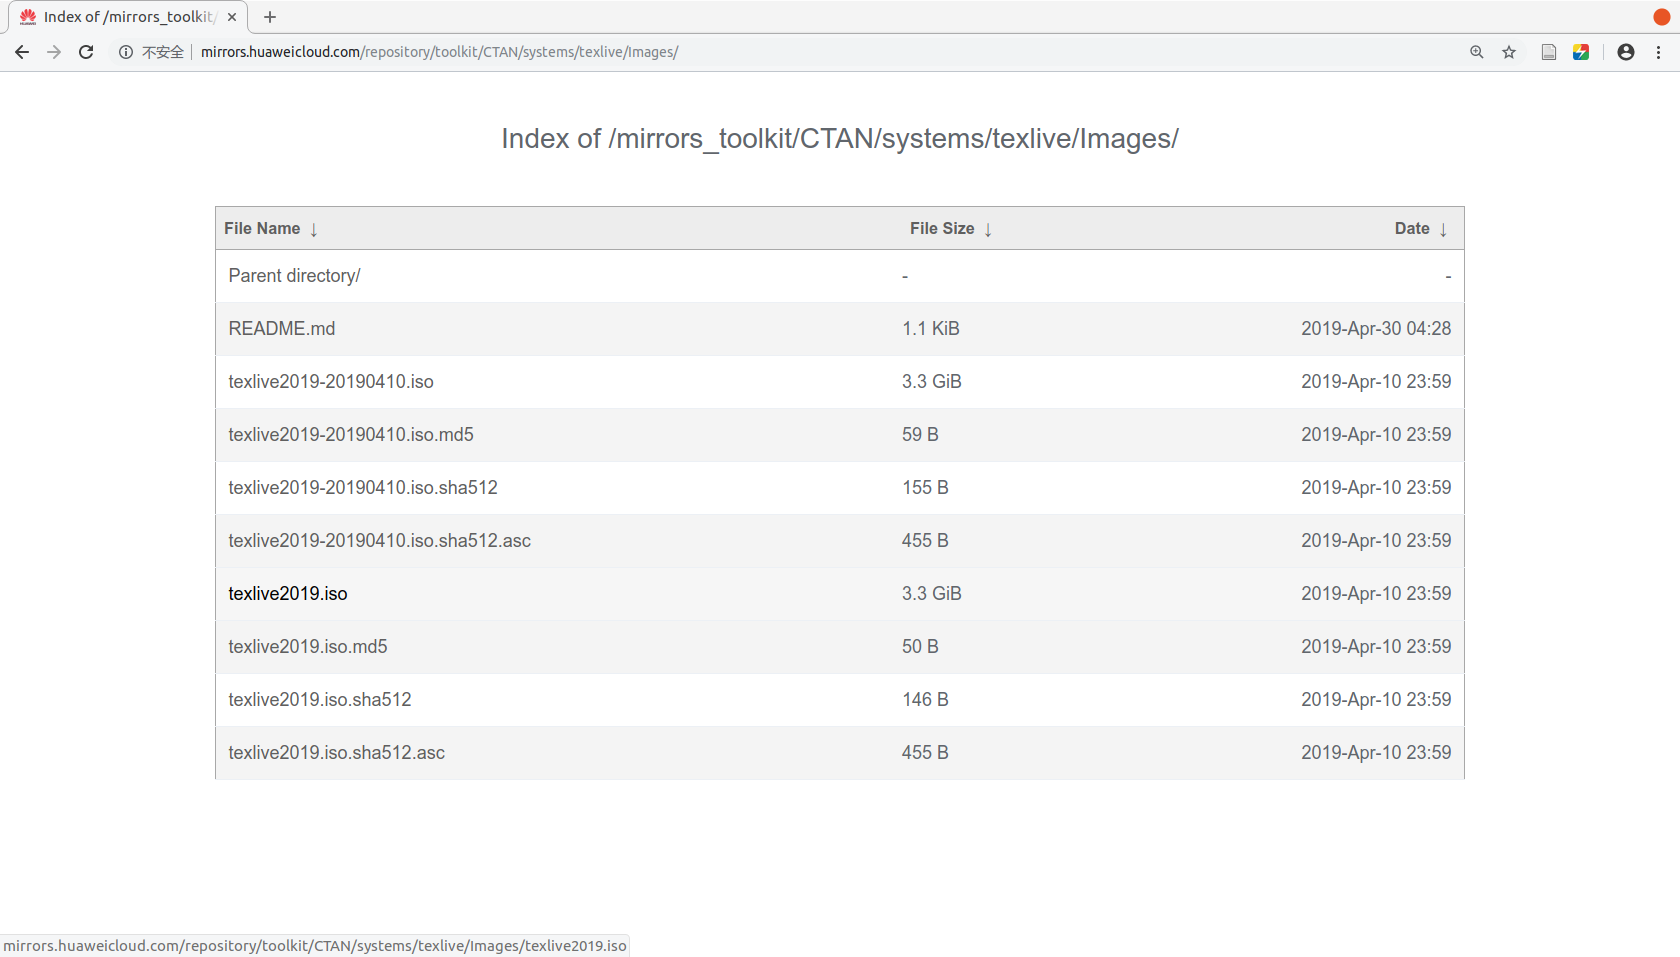
\includegraphics[width=0.95\textwidth]{downloadiso/isofilelist}}
    \annotatedFigureBox{0.125,0.357}{0.875,0.40}{blue}
    \annotatedFigureBox{0.528,0.36}{0.578,0.397}{red}
    \annotatedFigureBox{0.125,0.579}{0.875,0.622}{green}
    \annotatedFigureBox{0.528,0.582}{0.578,0.619}{red}
  \end{annotatedFigure}
\end{frame}

\begin{frame}{下载\TeXLive}{ISO镜像文件}
  %\stretchon
  \begin{itemize}
  \item 下载
    \begin{itemize}
    \item
      http://www.tug.org/texlive/\link{http://www.tug.org/texlive/}
      \begin{itemize}
      \item 开始下载
      \end{itemize}      
    \end{itemize}
  \end{itemize}
  \centering
  \vfill
  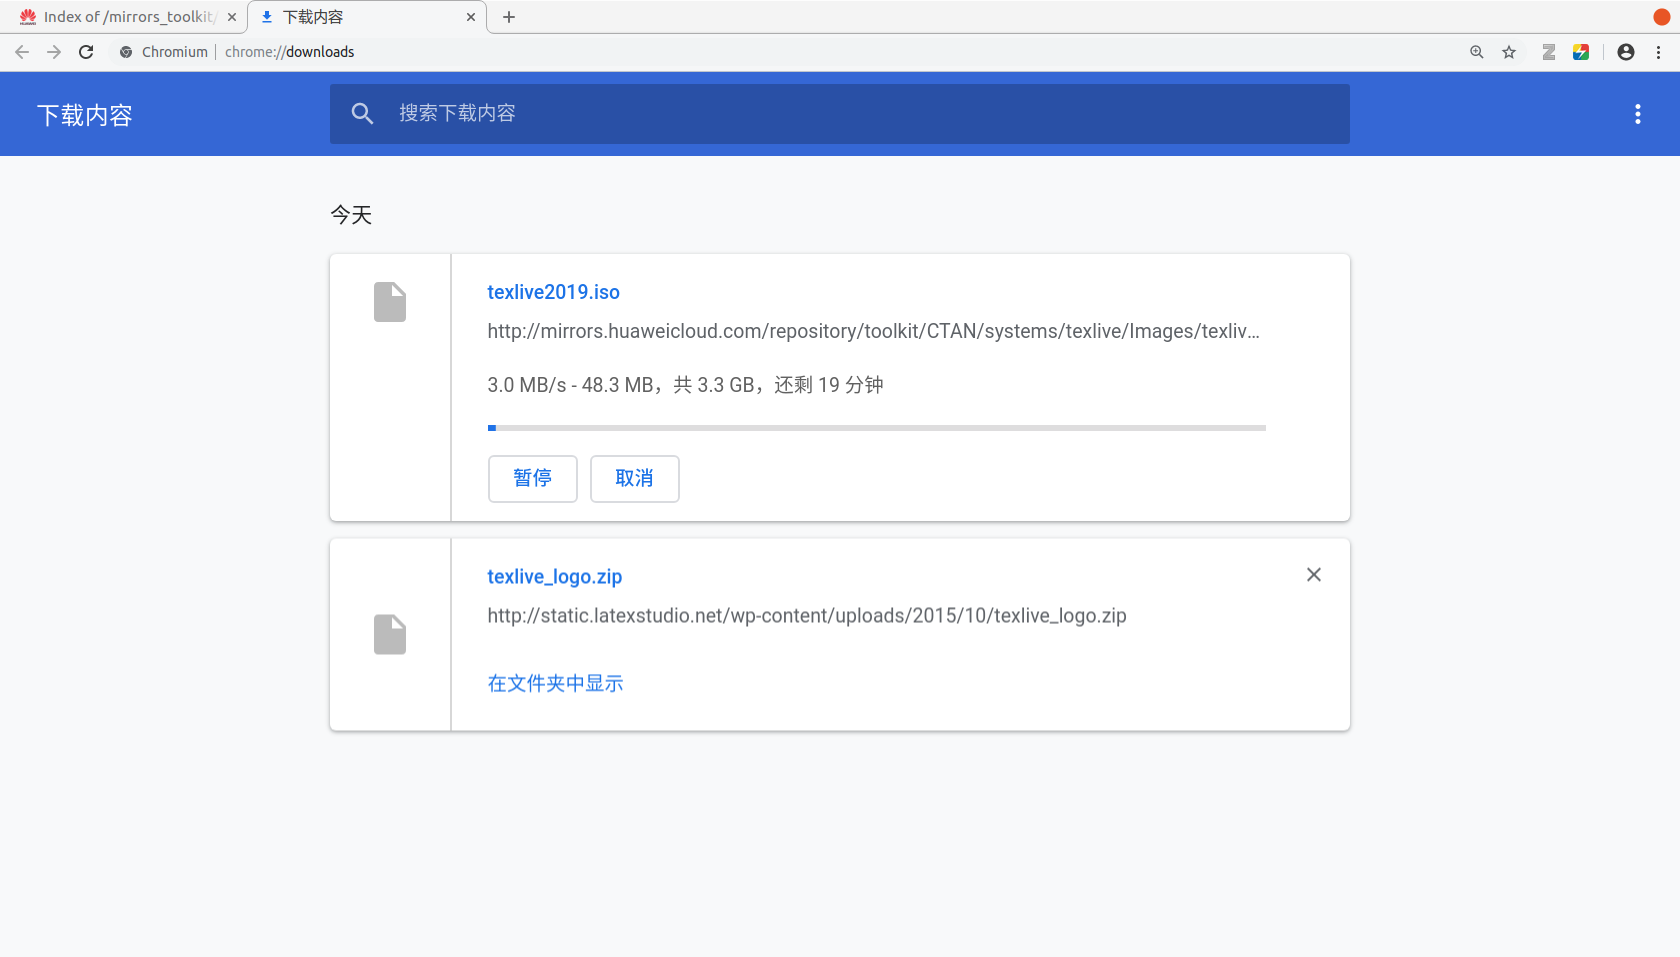
\includegraphics[width=0.85\textwidth]{downloadiso/isodownloading}
  \vfill
  %\stretchoff
\end{frame}
\begin{frame}[standout,plain]
  Downloading...
\end{frame}

\section[安装\TeXLive]{安装\TeXLive}
\subsection[命令行基础]{命令行基础}
\begin{frame}[fragile]{安装\tl}{命令行基础\footnote[frame,1]{本页面摘自曾祥东的\enquote{现代\LaTeX 入门讲座}讲义\link{https://github.com/stone-zeng/latex-talk}。}}
  % \footnote[frame,1]{本页面摘自曾祥东的\enquote{现代\LaTeX 入门讲座}讲义\link{https://github.com/stone-zeng/latex-talk}。}
  \begin{spacing}{1.25}
  \begin{itemize}
  \item 打开终端
    \begin{itemize}
      \setmenukeyswin
      \item \faWindows{}:右键开始菜单、空白处\keys{\shift + 右键}、\keys{\winmenu + R} \& \keys{cmd}
      \item \faLinux{}:\keys{\ctrl + \Alt + T}%\kbd{Ctrl} + \kbd{Alt} + \kbd{T}
      \setmenukeysmac  
      \item \faApple{}:\keys{\cmd + \Space} 搜索 Terminal、可在 Finder 中添加服务
    \end{itemize}
  \item 基本命令:
    \begin{itemize}
      \item \texinline{cd}、\texinline{ls/dir}、\texinline{rm/del}、\texinline{clear/cls}
      \item 选项:\texinline{-h}、\texinline{--help}、\texinline{/?}
    \end{itemize}
  \item 其他:
    \begin{itemize}
      \item 复制粘贴:\setmenukeyswin \keys{\ctrl /\shift + Ins}、
        \keys{\ctrl + c/v}、\setmenukeysmac \keys{\cmd + c/v}
      \item 路径连接符:斜线(\texinline{/})或反斜线(\texinline{\})
      \item 换行符:LF(\texinline{\n})或 CRLF(\texinline{\r\n})
      \item 结束进程:\setmenukeyswin \keys{\ctrl + C}
    \end{itemize} 
  \item 文件路径及命名中\alert{不要使用}中文、空格以及特殊符号
  \end{itemize}
  \end{spacing}
% \nonumberfootnote{本页摘自曾祥东的\enquote{现代\LaTeX 入门讲座}
%       讲义\link{https://github.com/stone-zeng/latex-talk}。}  
\end{frame}

\begin{frame}[fragile]{安装\tl}{命令行基础}
  %\begin{spacing}{1.5}
    \begin{itemize}
    \item Windows命令行窗口:\setmenukeyswin \keys{\winmenu + R}/小娜/
      开始 \& \keys{cmd}\\
      \begin{center}
        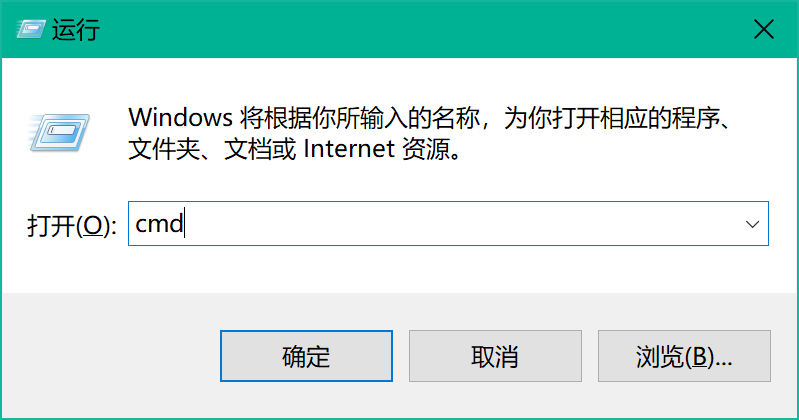
\includegraphics[height=0.32\textheight]{win10/00cmd01}
        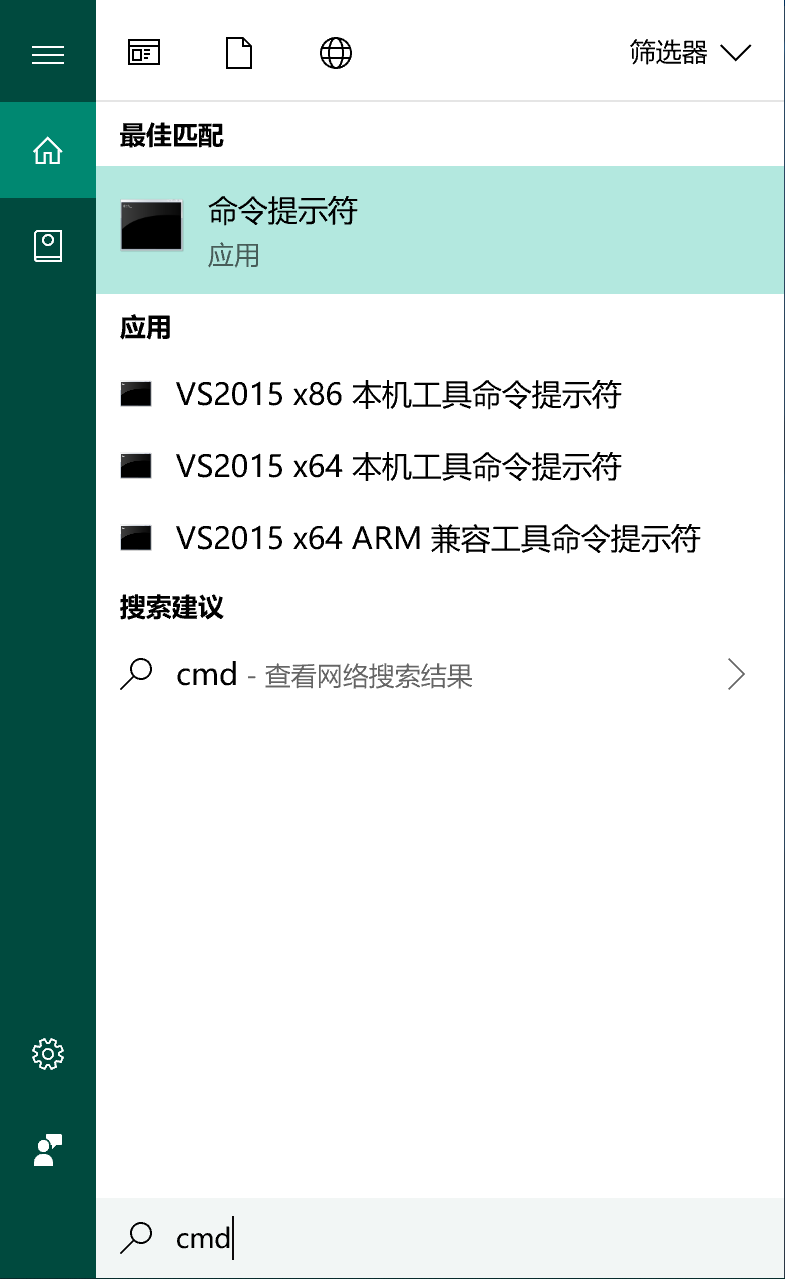
\includegraphics[height=0.32\textheight]{win10/00cmd02}
        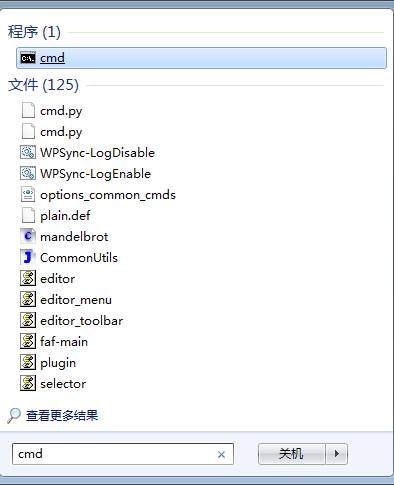
\includegraphics[height=0.32\textheight]{win7/00opencmd}\\
        \begin{minipage}[h]{0.95\linewidth}
          \windarkfile{显示当前目录中的文件}{datas/test.bat}
        \end{minipage}
      \end{center}    
    \end{itemize}
  %\end{spacing}
\end{frame}

\begin{frame}[fragile]{安装\tl}{命令行基础}
  %\begin{spacing}{1.5}
    \begin{itemize}
    \item Ubuntu终端窗口:\setmenukeyswin \keys{\ctrl + \Alt + T}\\
      \begin{center}
        \begin{minipage}[h]{0.9\linewidth}
          % 用命令排版,内容来自文件
          \ubtdarkfile{xxxxxx@xxxxxx-lap:~}{datas/ubtterm.sh}
        \end{minipage}
      \end{center}
    \item MacOS终端窗口:\setmenukeysmac \keys{\cmd +
        \Space} 搜索Terminal\\
      \begin{center}
        \begin{minipage}[h]{0.9\linewidth}
          % 用命令排版,内容来自文件
          \macdarkfile{xxxxxx@lap:~}{datas/macsh}
        \end{minipage}
      \end{center}
    \end{itemize}
  %\end{spacing}
\end{frame}

\subsection[Windows平台]{Windows平台下安装\tl}
\begin{frame}{安装\tl}{装备安装文件}
  \begin{spacing}{1.0}
    \begin{itemize}
    \item 加载\enquote{texlive2019.iso}文件
      \begin{itemize}
      \item Win10直接装载或用虚拟光驱加载
      \item Win7及其它用虚拟光驱加载
      \end{itemize}      
    \item 解压\enquote{texlive2019.iso}文件
    \end{itemize}
  %\end{spacing}
  \begin{center}
    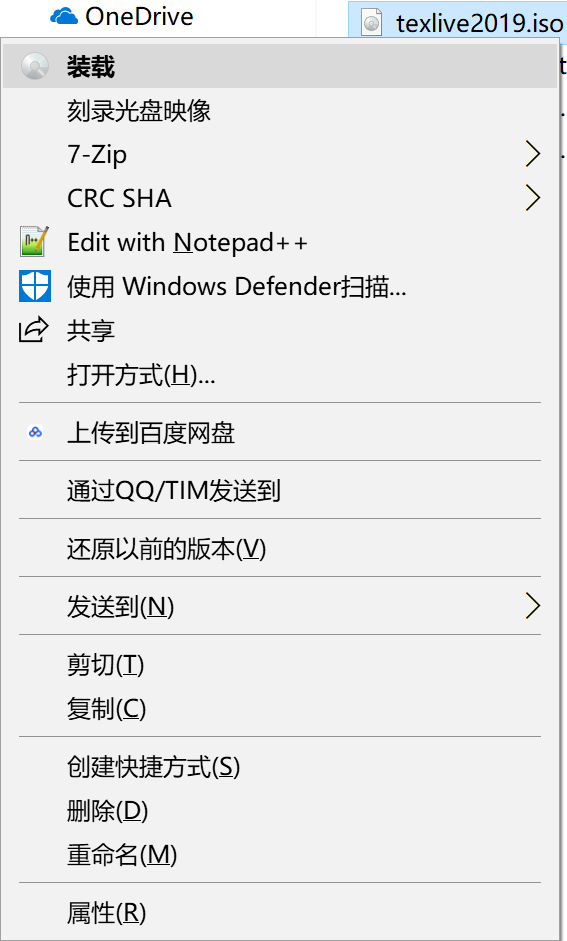
\includegraphics[height=0.5\textheight]{win10/00rightclickisowin10}
    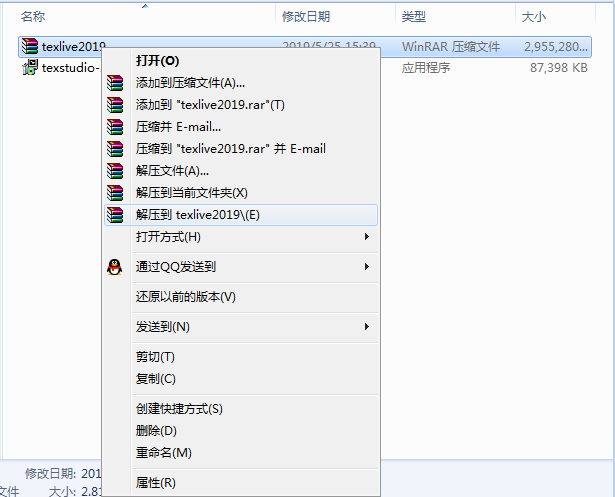
\includegraphics[height=0.5\textheight]{win7/00downloadtl2019-10}
    %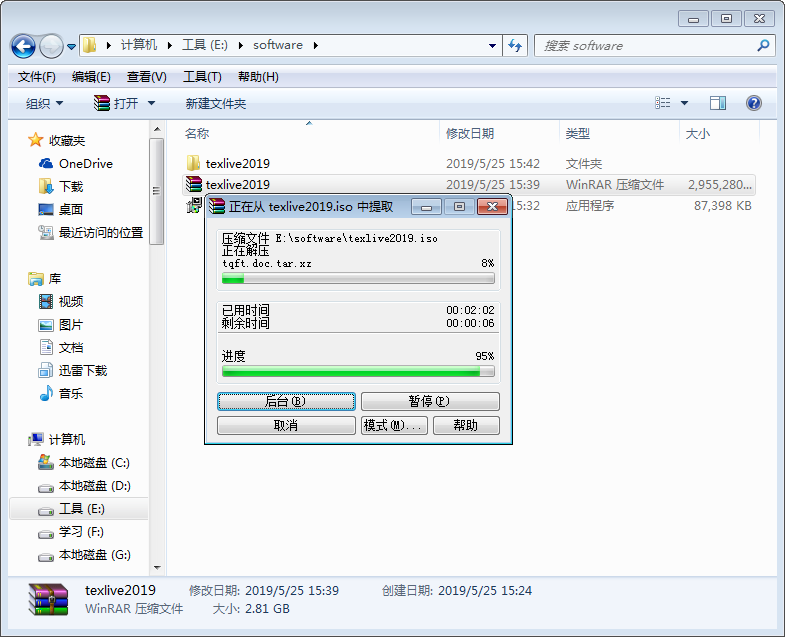
\includegraphics[height=0.5\textheight]{win7/00downloadtl2019-15}
  \end{center}
  \end{spacing}
\end{frame}

\begin{frame}[standout,plain]
  解压...
\end{frame}

\begin{frame}{安装\tl}{装备安装文件}
  \begin{spacing}{1.0}
    \begin{itemize}
    \item 得到\alert{安装文件}
    \end{itemize}  
  \begin{center}    
    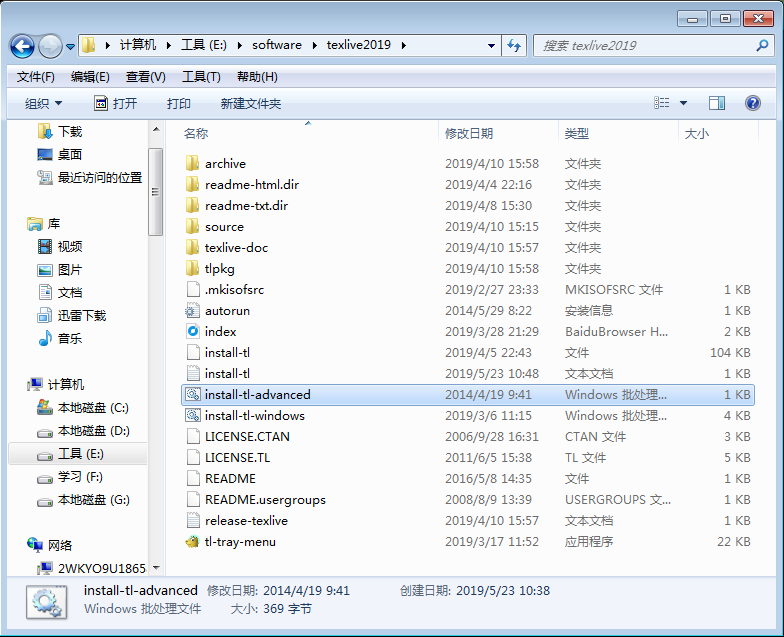
\includegraphics[height=0.7\textheight]{win7/00TexLive2019files}
  \end{center}
  \end{spacing}
\end{frame}

\begin{frame}{安装\tl}{Windows平台}
  \begin{spacing}{1.0}
    \begin{itemize}
    \item 双击\enquote{install-tl-advanced}文件启动\TeXLive 安装
    \end{itemize}  
  \begin{center}    
    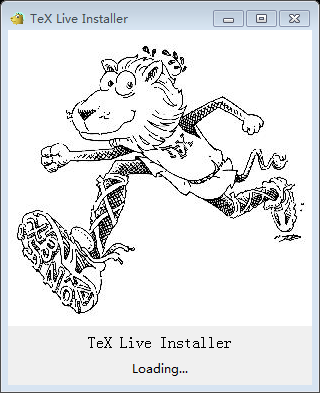
\includegraphics[height=0.55\textheight]{win7/01loading}
    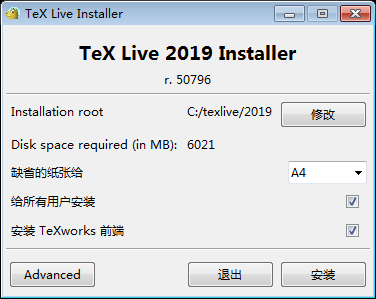
\includegraphics[height=0.55\textheight]{win7/02installer}
  \end{center}
  \end{spacing}
\end{frame}

\begin{frame}{安装\tl}{Windows平台}
  \begin{spacing}{1.8}
    \begin{itemize}
    \item 单击\enquote{Installation root}后的\keys{修改}按钮可更改\alert{安装根目录}
    \end{itemize}  
    \begin{center}
      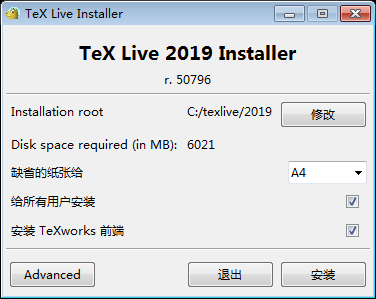
\includegraphics[height=0.35\textheight]{win7/02installer}
      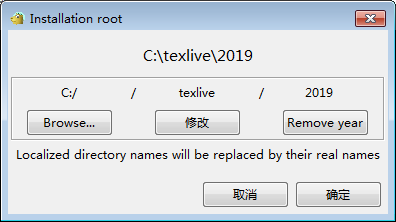
\includegraphics[height=0.35\textheight]{win7/03changedir}
    \end{center}
  \end{spacing}
\end{frame}

\begin{frame}{安装\tl}{Windows平台}
  \begin{spacing}{1.8}
    \begin{itemize}
    \item 单击\keys{Advanced}按钮可定制安装选项
    \end{itemize}  
    \begin{center}
      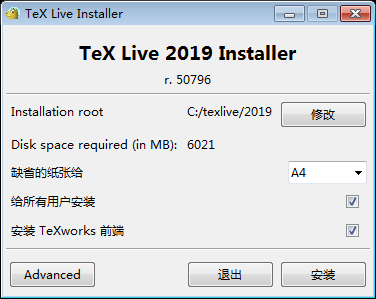
\includegraphics[height=0.4\textheight]{win7/02installer}
      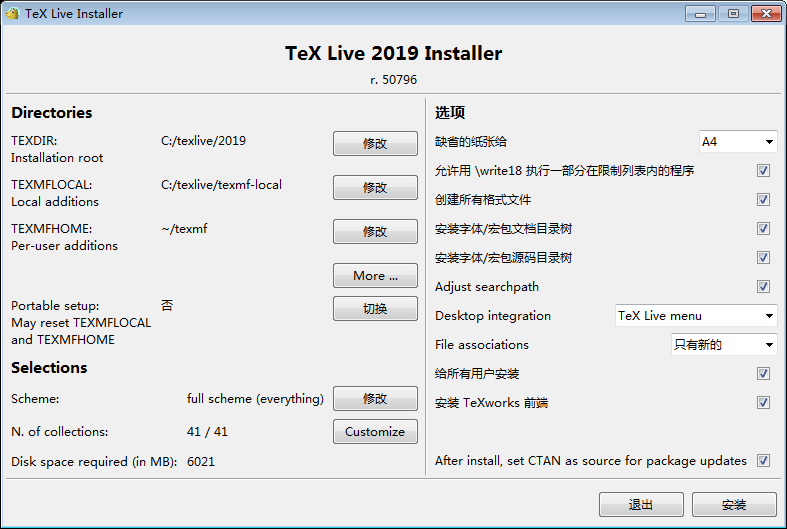
\includegraphics[height=0.4\textheight]{win7/03defaultsettings}
    \end{center}
  \end{spacing}
\end{frame}

\begin{frame}{安装\tl}{Windows平台}
  \begin{spacing}{1.8}
    \begin{itemize}
    \item 单击\enquote{Scheme}后的\keys{修改}按钮可选择安装方案
    \end{itemize}  
    \begin{center}
      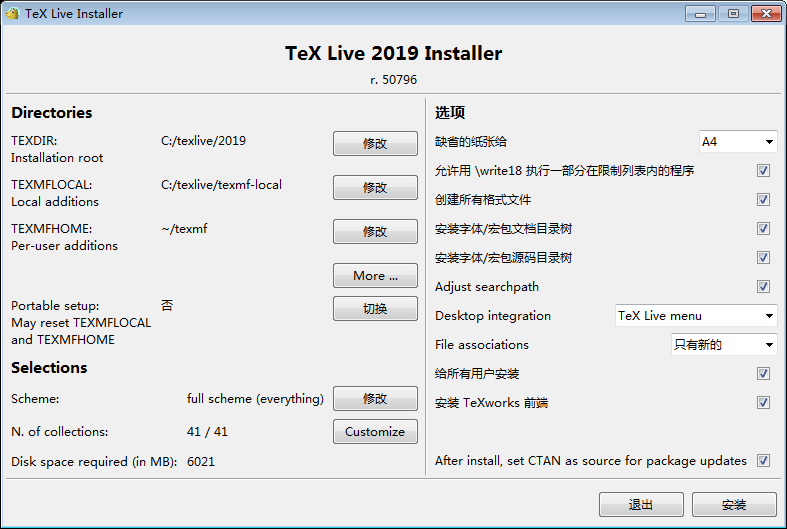
\includegraphics[height=0.5\textheight]{win7/03defaultsettings}
      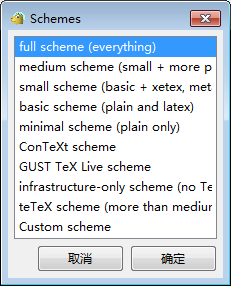
\includegraphics[height=0.5\textheight]{win7/05installschemes}
    \end{center}
  \end{spacing}
\end{frame}

\begin{frame}{安装\tl}{Windows平台}
  \begin{spacing}{1.8}
    \begin{itemize}
    \item 单击\enquote{collections}后的\keys{Customize}按钮可选择安装
      宏包\footnote[frame,1]{建议完整安装宏包,以备不时之需。}
    \end{itemize}  
    \begin{center}
      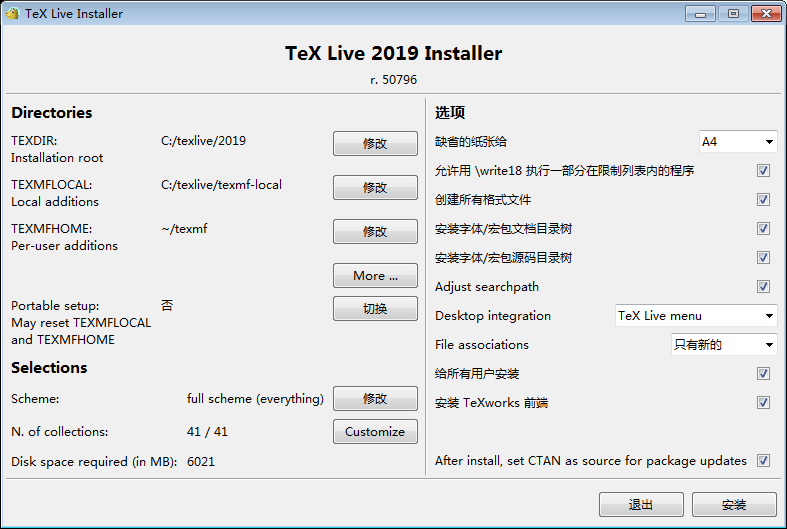
\includegraphics[height=0.38\textheight]{win7/03defaultsettings}
      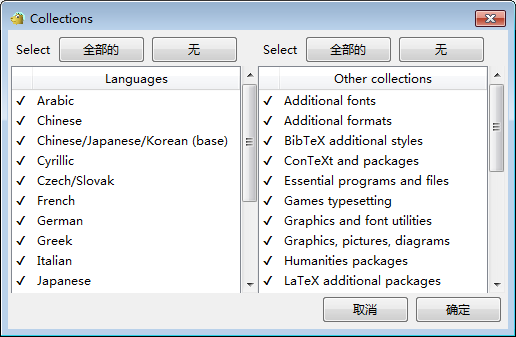
\includegraphics[height=0.38\textheight]{win7/05installschemescustom}
    \end{center}
  \end{spacing}
\end{frame}

\begin{frame}{安装\tl}{Windows平台}
  \begin{spacing}{1.0}
    \begin{itemize}
    \item 完成定制后单击\keys{安装}进行\tl 安装
    \end{itemize}  
    \begin{center}
      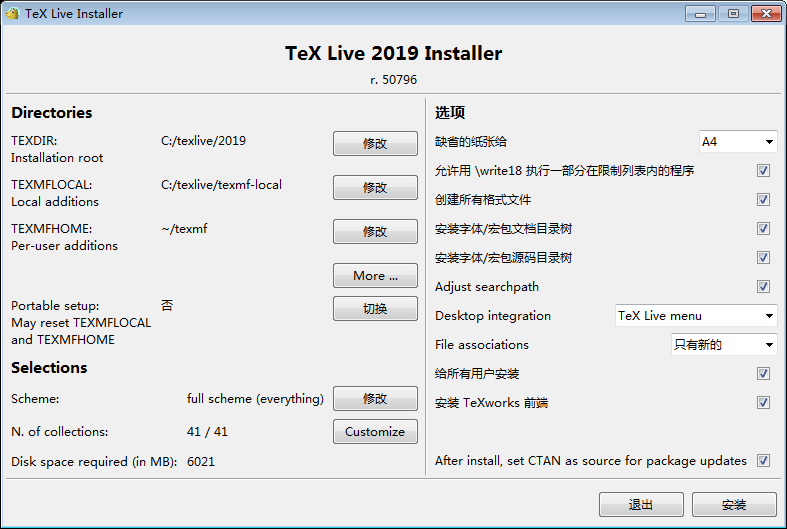
\includegraphics[width=0.58\textwidth]{win7/03defaultsettings}\\
      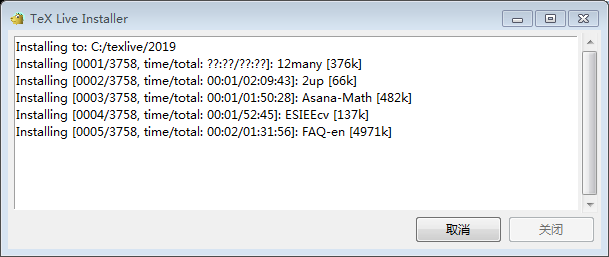
\includegraphics[width=0.58\textwidth]{win7/06installing00}
    \end{center}
  \end{spacing}
\end{frame}

\begin{frame}[standout,plain]
  安装...
\end{frame}

\begin{frame}{安装\tl}{Windows平台}
  \begin{spacing}{1.0}
    \begin{itemize}
    \item 单击\keys{关闭}完成\tl 安装
    \end{itemize}  
    \begin{center}
      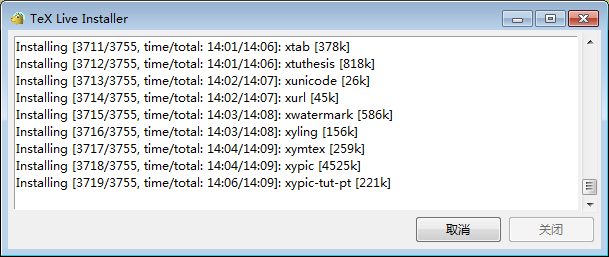
\includegraphics[width=0.68\textwidth]{win7/06installing08}\\
      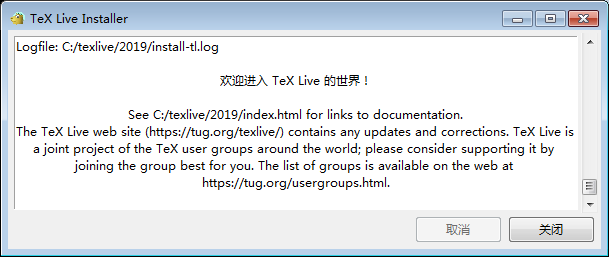
\includegraphics[width=0.68\textwidth]{win7/06installing14}
    \end{center}
  \end{spacing}
\end{frame}

\begin{frame}{安装\tl}{Windows平台}
  \begin{spacing}{1.5}
    \begin{itemize}
    \item 检查\tl 是否安装成功
      \begin{itemize}
      \item 打开命令行,输入:xelatex -v
        \begin{itemize}
        \item 正常:输出\alert{版本}信息
          \begin{center}
            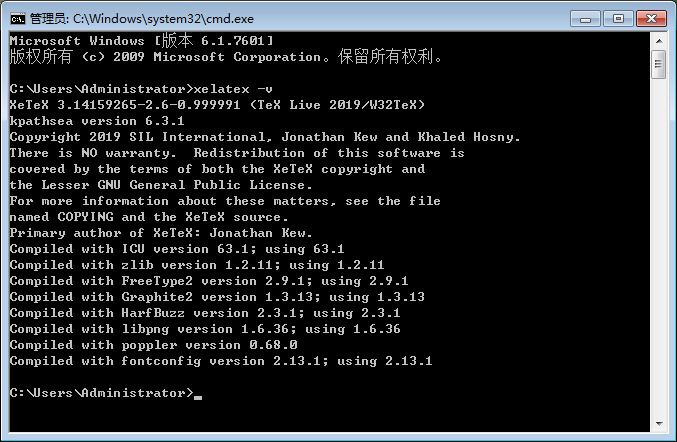
\includegraphics[width=0.75\textwidth]{win7/07xelatex-v-cmd}
          \end{center}
        \end{itemize}
      \end{itemize}
    \end{itemize}
  \end{spacing}         
\end{frame}

\begin{frame}{安装\tl}{Windows平台}
  \begin{spacing}{1.5}
    \begin{itemize}
    \item 检查\tl 是否安装成功
      \begin{itemize}
      \item 打开命令行,输入:xelatex -v
        \begin{itemize}
        \item 错误:输出\alert{命令错误},一般是\alert{环境变量}配置错误造成的
          \begin{center}
            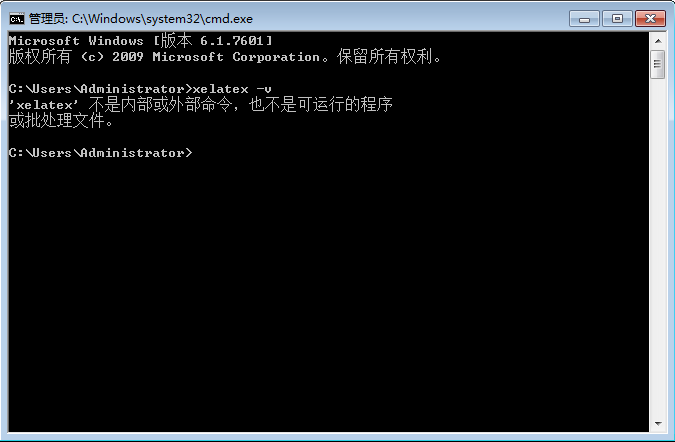
\includegraphics[width=0.75\textwidth]{win7/09cmderror}
          \end{center}
        \end{itemize}
      \end{itemize}
    \end{itemize}
  \end{spacing}         
\end{frame}

\begin{frame}{安装\tl}{Windows平台}
  \begin{spacing}{1.5}
    \begin{itemize}
    \item 环境变量
      \begin{itemize}
      \item 右击桌面上\enquote{ThePC}(Win10)或\enquote{我的电脑}(Win7)
        \begin{itemize}
        \item 选择\keys{属性}打开系统属性对话框          
        \end{itemize}
      \end{itemize}
    \end{itemize}
    \begin{center}
      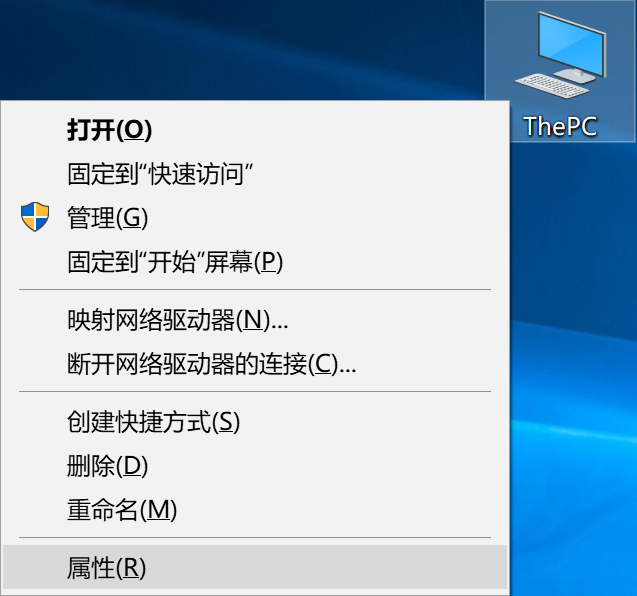
\includegraphics[height=0.42\textheight]{win10/00rightclickthepc}
      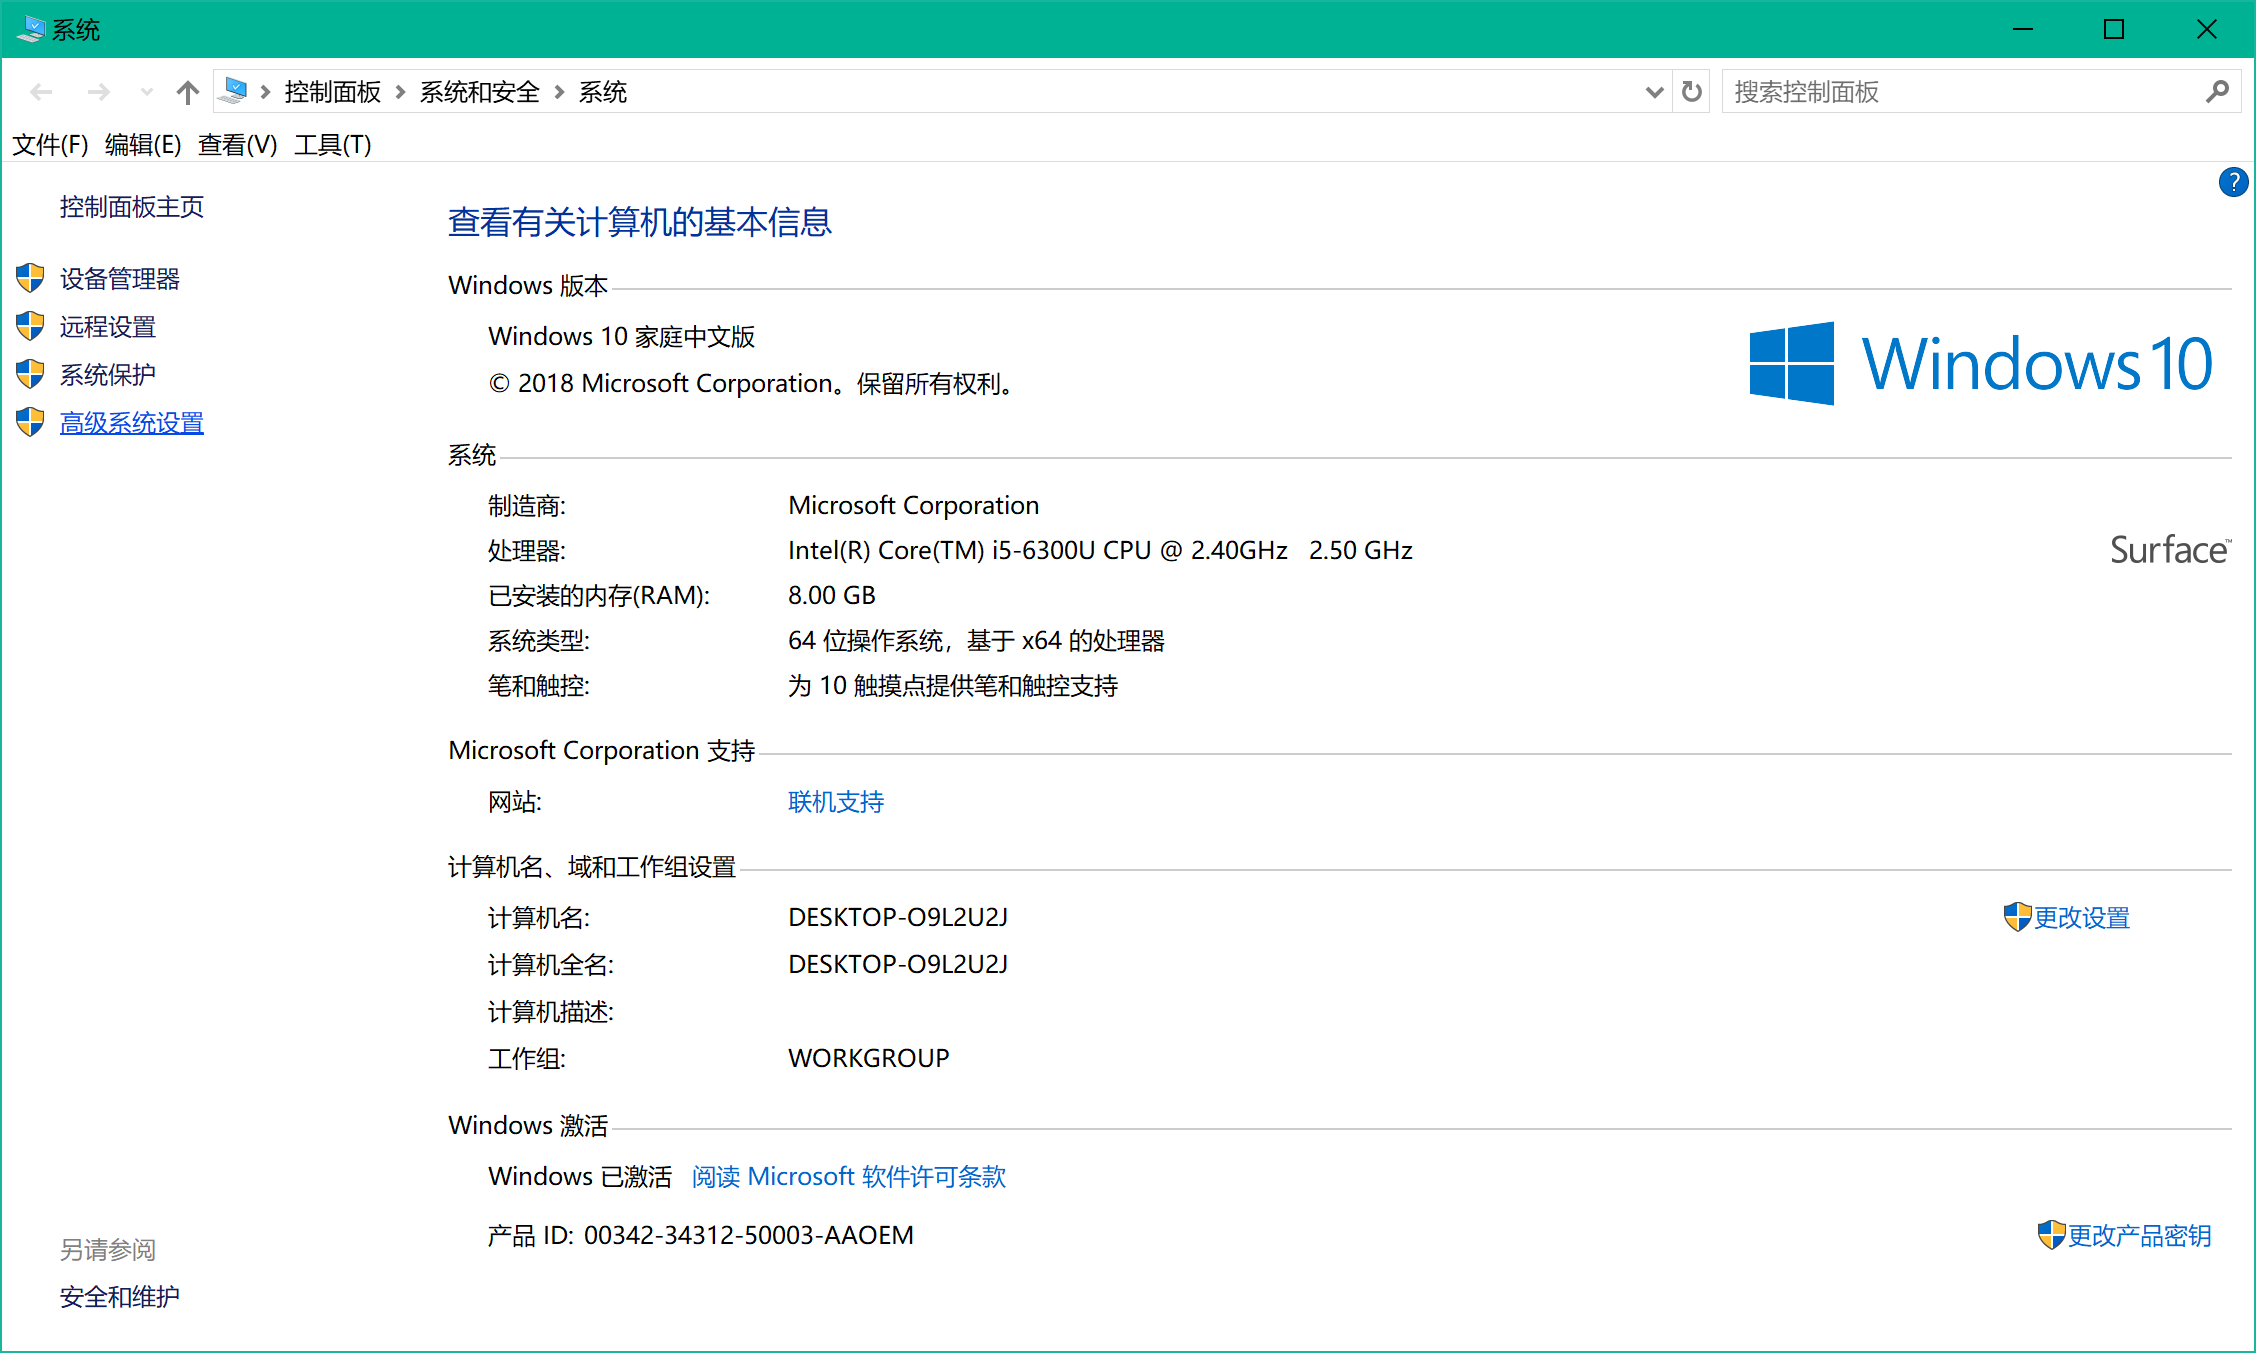
\includegraphics[height=0.42\textheight]{win10/01pathsettings01beforeinst}
    \end{center}
  \end{spacing}         
\end{frame}

\begin{frame}{安装\tl}{Windows平台}
  \begin{spacing}{1.5}
    \begin{itemize}
    \item 环境变量
      \begin{itemize}
      \item 环境变量对话框
        \begin{itemize}
        \item 选择\keys{高级系统设置}打开系统属性对话框
        \item 在系统属性对话框中\keys{环境变量}打开环境变量对话框
        \item 可以对当前用户设置,也可以对系统用户进行设置
        \end{itemize}
      \end{itemize}
    \end{itemize}
    \begin{center}
      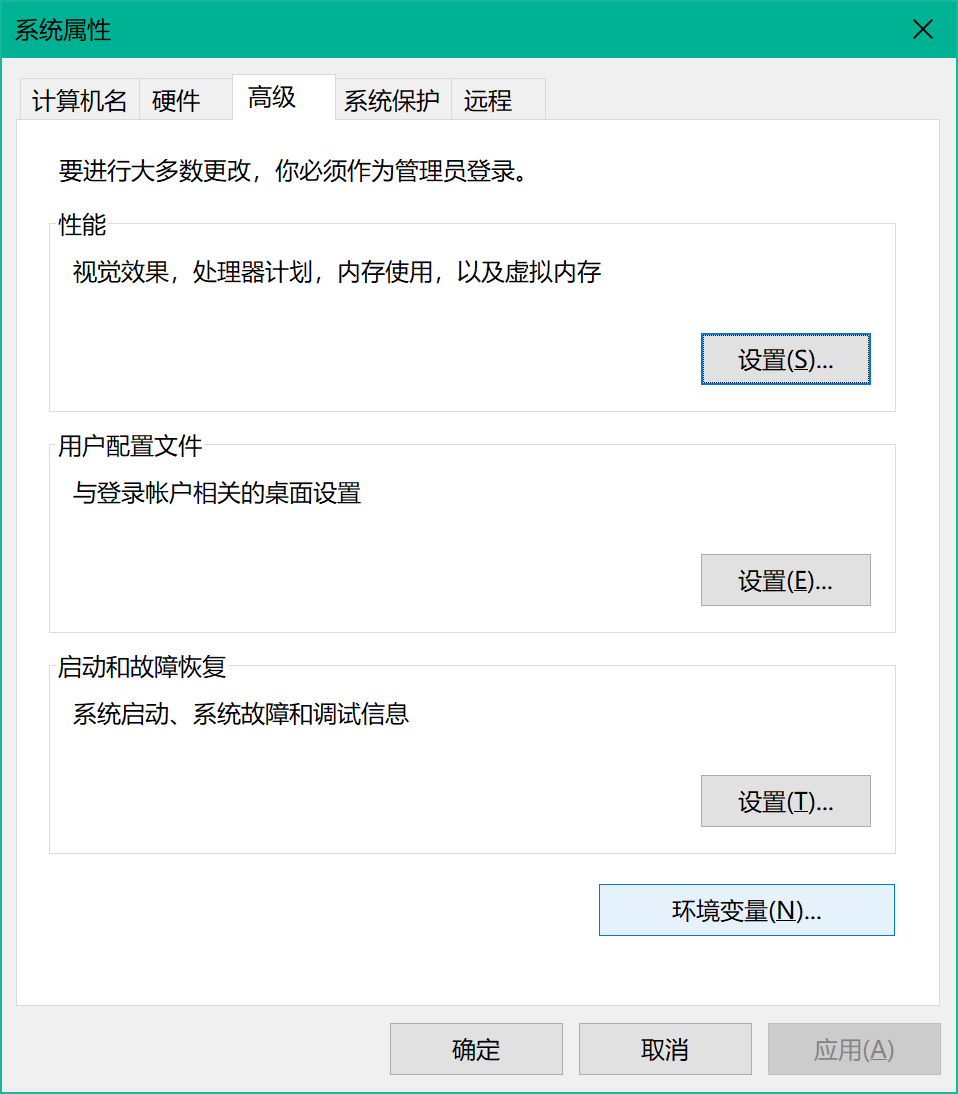
\includegraphics[height=0.4\textheight]{win10/01pathsettings01beforeins02t}
      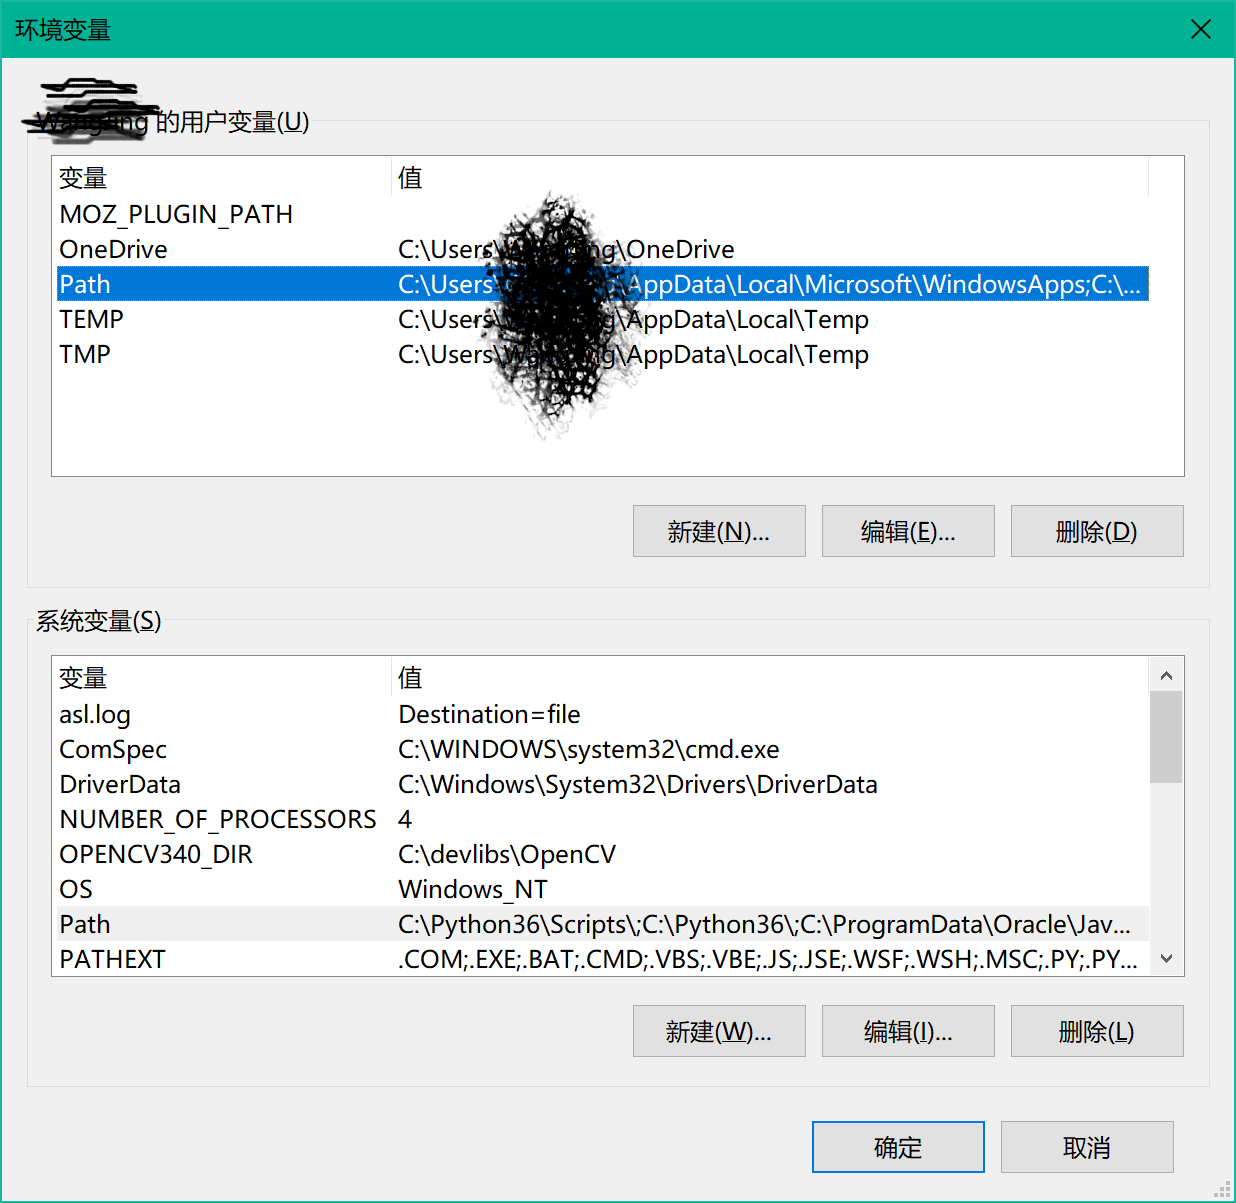
\includegraphics[height=0.4\textheight]{win10/05texlive2019instdonepath01}
      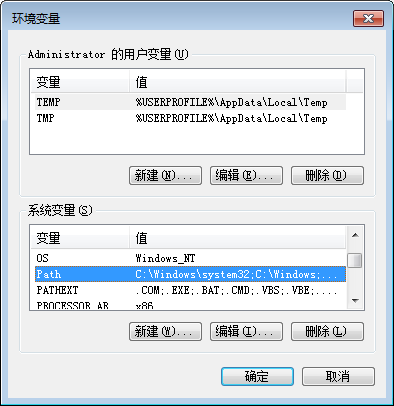
\includegraphics[height=0.4\textheight]{win7/05pathsettingbeforeinst}
    \end{center}
  \end{spacing}         
\end{frame}

\begin{frame}{安装\tl}{Windows平台}
  \begin{spacing}{1.2}
    \begin{itemize}
    \item 环境变量
      \begin{itemize}
      \item 双击\enquote{Path}环境变量进行设置(Win10)
        \begin{itemize}
        \item 通过\keys{新建}按钮创建环境变量
        \item 通过\keys{编辑}按钮编辑环境变量
        \item 将\enquote{\tl}的\enquote{bin}安装路径添加到环境变量          
        \end{itemize}
      \end{itemize}
    \end{itemize}
    \begin{center}
      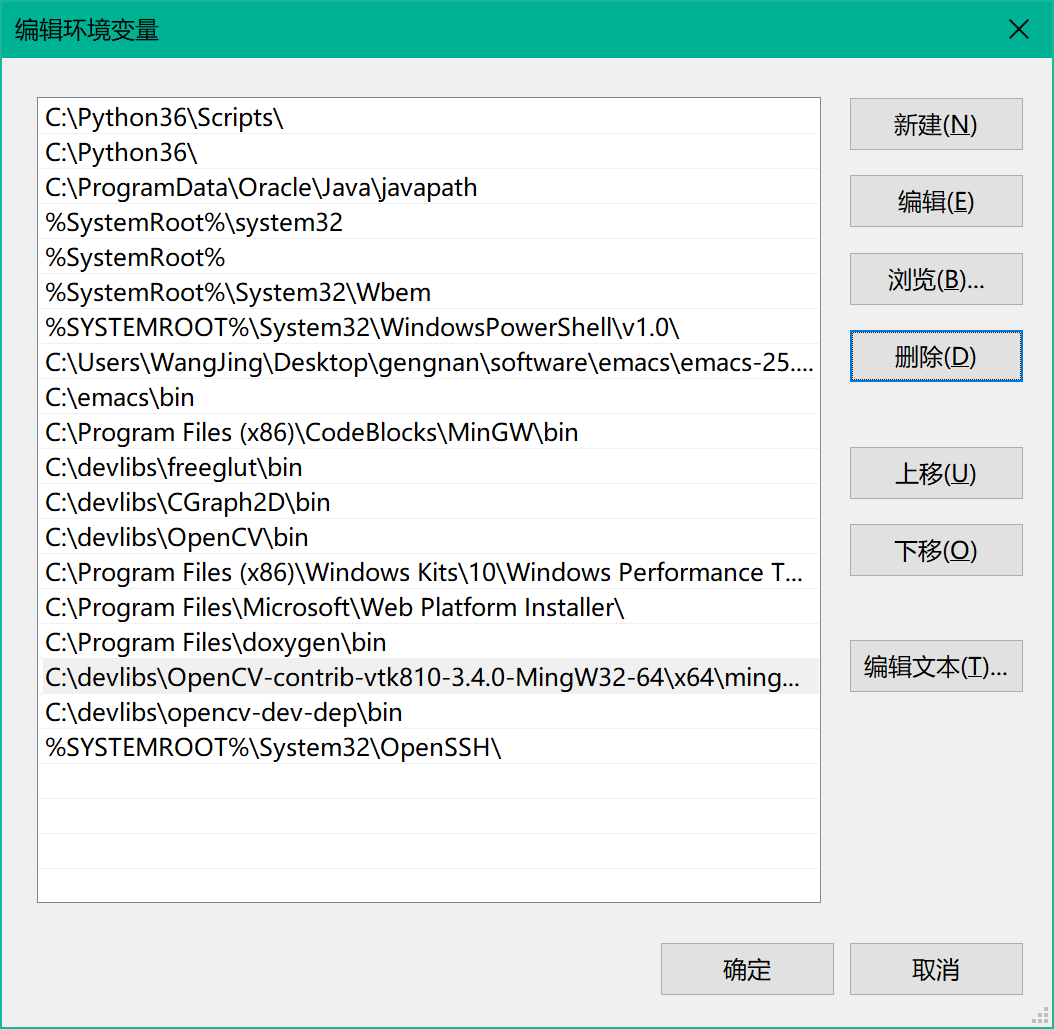
\includegraphics[height=0.5\textheight]{win10/01pathsettings01beforeinst03}
      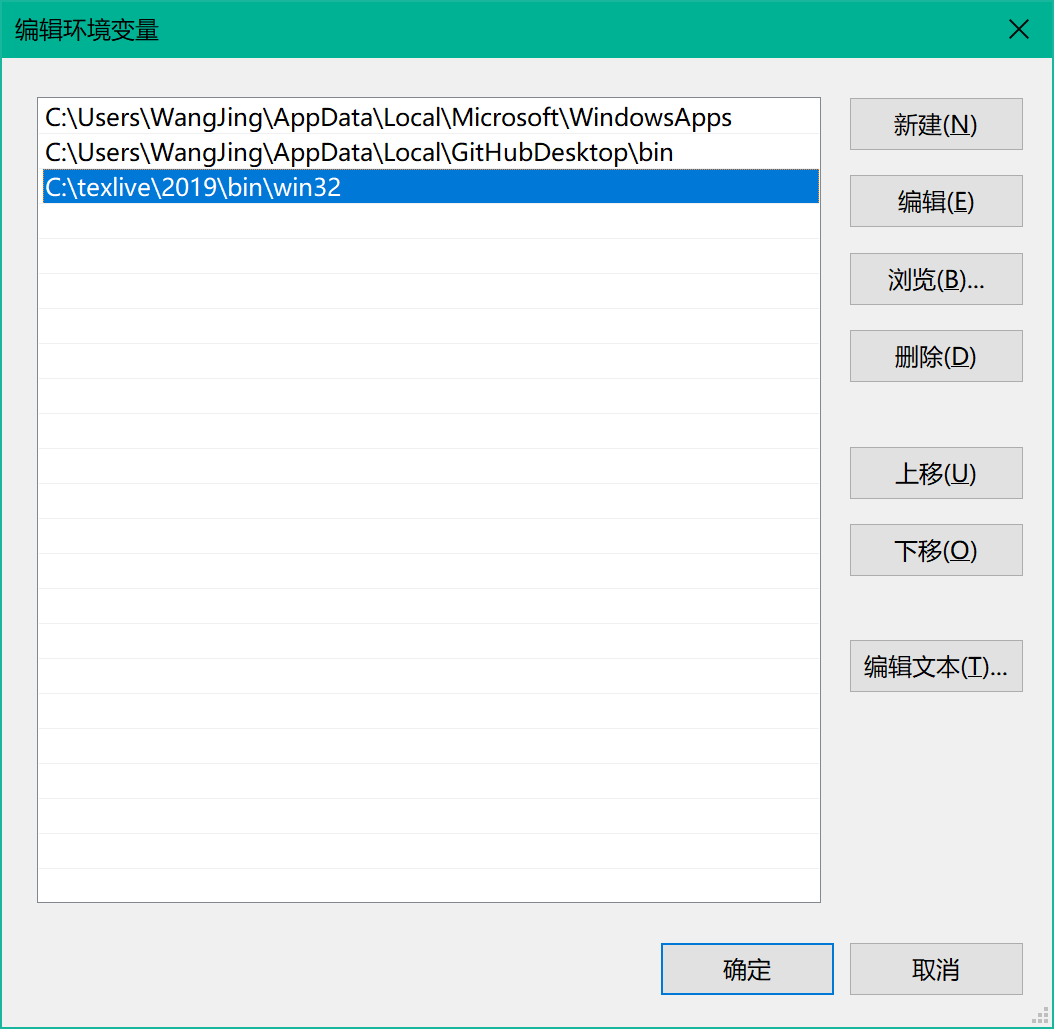
\includegraphics[height=0.5\textheight]{win10/05texlive2019instdonepath03}
    \end{center}
  \end{spacing}         
\end{frame}

\begin{frame}{安装\tl}{Windows平台}
  \begin{spacing}{1.5}
    \begin{itemize}
    \item 环境变量
      \begin{itemize}
      \item 双击\enquote{Path}环境变量进行设置(Win7)
        \begin{itemize}
        \item 将\enquote{\tl}的\enquote{bin}安装路径添加到环境变量
        \end{itemize}
      \end{itemize}
    \end{itemize}
    \begin{center}
      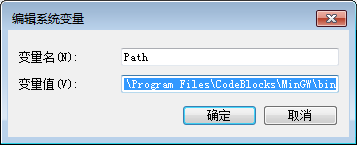
\includegraphics[height=0.3\textheight]{win7/05pathsettingbeforeinst2}\\
      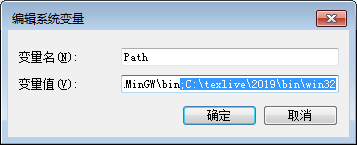
\includegraphics[height=0.3\textheight]{win7/07pathsettingafterinst}
    \end{center}
  \end{spacing}         
\end{frame}

\begin{frame}{安装\tl}{Windows平台}
  \begin{spacing}{1.5}
    \begin{itemize}
    \item 环境变量
      \begin{itemize}
      \item 需确保\enquote{\tl}的\enquote{bin}路径正确
        \begin{itemize}
          \renewmenumacro{\directory}{pathswithfolder} % default: paths
        \item 默认:\directory[,]{C:,texlive,2019,bin,win32}
        \item \enquote{\alert{xelatex.exe}}等可执行文件所在的路径
        \end{itemize}
      \end{itemize}
    \end{itemize}
    \begin{center}
      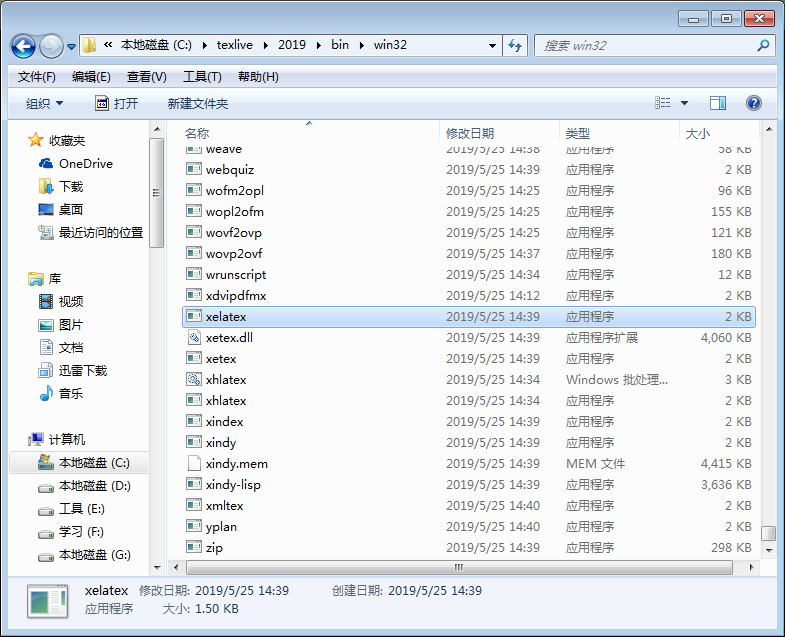
\includegraphics[height=0.5\textheight]{win7/07binpath}
    \end{center}
  \end{spacing}         
\end{frame}

\begin{frame}{安装\tl}{Windows平台}
  \begin{spacing}{1.5}
    \begin{itemize}
    \item 环境变量
      \begin{itemize}
      \item 也可以在命令行用\enquote{path}命令查看环境变量
      \end{itemize}
    \end{itemize}
    \begin{center}
      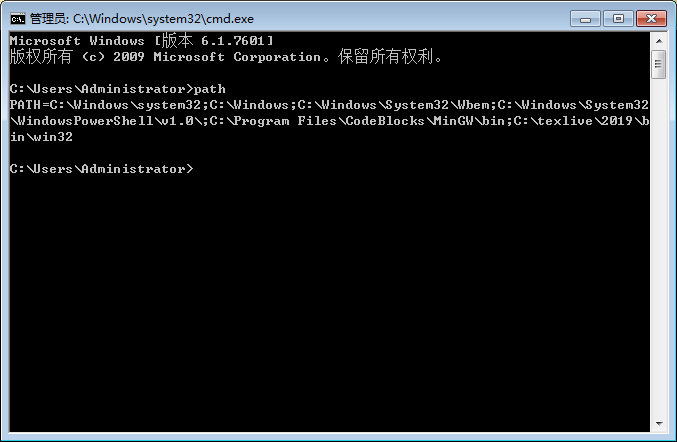
\includegraphics[height=0.65\textheight]{win7/07pathsettingcmd}
    \end{center}
  \end{spacing}         
\end{frame}

\begin{frame}[standout,plain]
  如果环境变量正确,还无法执行\enquote{xelatex -v},\\那就重装\tl 吧!
\end{frame}

\subsection[Ubuntu平台]{Ubuntu平台下安装\tl}
\begin{frame}{安装\tl}{Ubuntu平台}
  \begin{spacing}{1.0}
    \begin{itemize}
    \item 图形化安装界面需安装\enquote{perl}的\enquote{tk}组件
      \begin{itemize}
      \item 打开终端:\setmenukeyswin \keys{\ctrl + \Alt + T}\\
      \item 执行:\shinline{sudo apt-get install perl-tk}
      \end{itemize}
    \end{itemize}
  \begin{center}
    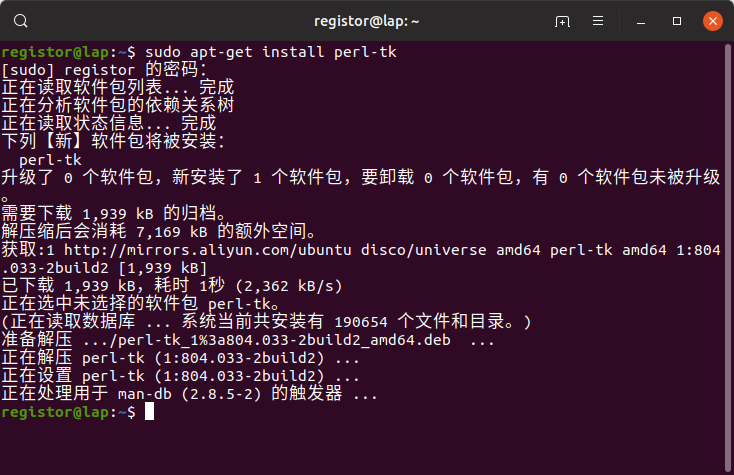
\includegraphics[height=0.6\textheight]{ubuntu/01installperl-tk}
  \end{center}
  \end{spacing}
\end{frame}

\begin{frame}{安装\tl}{Ubuntu平台}
  \begin{spacing}{1.0}
    \begin{itemize}
    \item 加载\enquote{texlive2019.iso}镜像文件
      \begin{itemize}
      \item 打开终端:\setmenukeyswin \keys{\ctrl + \Alt + T}\\
      \item 执行:\shinline{sudo mount -o loop texlive2019.iso /mnt}
      \end{itemize}
    \end{itemize}
  \begin{center}
    \includegraphics[height=0.6\textheight]{ubuntu/02mountiso}
  \end{center}
  \end{spacing}
\end{frame}

\begin{frame}{安装\tl}{Ubuntu平台}
  \begin{spacing}{1.0}
    \begin{itemize}
    \item 启动\tl 图形化安装界面
      \begin{itemize}
      \item 打开终端:\setmenukeyswin \keys{\ctrl + \Alt + T}
      \item 执行:\shinline{cd /mnt}
      \item 执行:\shinline{sudo ./install-tl -gui}
      \end{itemize}
    \end{itemize}
  \begin{center}
    \includegraphics[height=0.45\textheight]{ubuntu/03install-tl-guicmd}
    \includegraphics[height=0.45\textheight]{ubuntu/04installgui}
  \end{center}
  \end{spacing}
\end{frame}

\begin{frame}{安装\tl}{Ubuntu平台}
  \begin{spacing}{1.0}
    \begin{itemize}
    \item 选择\tl 安装方案及宏包组件\footnote[frame,1]{建议全部安装,
        以备不时之需。}
      \begin{itemize}
      \item 使用\keys{修改}按钮选择不同安装选项
      \end{itemize}
    \end{itemize}
  \begin{center}
    \includegraphics[height=0.5\textheight]{ubuntu/05installscheme}
    \includegraphics[height=0.5\textheight]{ubuntu/06packagelist}
  \end{center}
  \end{spacing}
\end{frame}

\begin{frame}{安装\tl}{Ubuntu平台}
  \begin{spacing}{1.0}
    \begin{itemize}
    \item 选择\tl 安装方案及宏包组件
      \begin{itemize}
      \item 可以更改安装路径
      \item 注意创建\alert{指向系统目录的符号链接}\footnote[frame,1]{否则无法正确执
        行各个编译命令。}
      \end{itemize}
    \end{itemize}
  \begin{center}
     \includegraphics[height=0.3\textheight]{ubuntu/07changedir}\\  
    \includegraphics[height=0.3\textheight]{ubuntu/07symbollink}
    %\includegraphics[height=0.5\textheight]{ubuntu/06packagelist}
  \end{center}
  \end{spacing}
\end{frame}

\begin{frame}{安装\tl}{Ubuntu平台}
  \begin{spacing}{1.0}
    \begin{itemize}
    \item 选择\tl 安装方案及宏包组件
      \begin{itemize}
      \item 确认无误后,单击\keys{安装\TeXLive}进行安装
      \end{itemize}
    \end{itemize}
    \begin{center}
      \begin{annotatedFigure}
        {\includegraphics[height=0.7\textheight]{ubuntu/08afterscheme}}
        \annotatedFigureBox{0.125,0.11}{0.995,0.15}{red}
      \end{annotatedFigure}
    \end{center}
  \end{spacing}
\end{frame}

\begin{frame}[standout,plain]
  安装...
\end{frame}

\begin{frame}{安装\tl}{Ubuntu平台}
  \begin{spacing}{1.5}
    \begin{itemize}
    \item 安装结束
      \begin{itemize}
      \item 单击\keys{完成}
      \end{itemize}
    \end{itemize}
  \begin{center}
    \includegraphics[height=0.6\textheight]{ubuntu/09installdone}
    %\includegraphics[height=0.5\textheight]{ubuntu/06packagelist}
  \end{center}
  \end{spacing}
\end{frame}

\begin{frame}{安装\tl}{Ubuntu平台}
  \begin{spacing}{1.5}
    \begin{itemize}
    \item 安装结束
      \begin{itemize}
      \item 单击\keys{完成}
      \item 卸载镜像文件:\shinline{cd /; sudo umount /mnt}
      \end{itemize}
    \end{itemize}
  \begin{center}
    \includegraphics[height=0.6\textheight]{ubuntu/09installdone}
    %\includegraphics[height=0.5\textheight]{ubuntu/06packagelist}
  \end{center}
  \end{spacing}
\end{frame}

\begin{frame}{安装\tl}{Ubuntu平台}
  \begin{spacing}{1.2}
    \begin{itemize}
    \item 检查\tl 是否安装成功
      \begin{itemize}
      \item 打开终端:\setmenukeyswin \keys{\ctrl + \Alt + T}
      \item 输入命令:xelatex -v
        \begin{itemize}
        \item 正常:输出\alert{版本}信息          
        \end{itemize}
      \end{itemize}
    \end{itemize}
    \begin{center}
      \includegraphics[width=0.75\textwidth]{ubuntu/10xelatex-v-cmd}
    \end{center}
  \end{spacing}
\end{frame}

\begin{frame}[standout,plain]
  如果无法执行\enquote{xelatex -v},那就重装\tl 吧!\\特别要注意的是
  \alert{创建符号链接}!
\end{frame}

\section[更新\TeXLive]{更新\tl}
\begin{frame}{更新\tl}{Windows/Ubuntu平台}
  \begin{spacing}{1.5}
    \begin{itemize}
    \item 执行\enquote{tlmgr}更新\tl %
      \begin{itemize}
      \item 打开命令行
      \item 输入命令:\shinline{tlmgr update --self --all}(Windows)
        \footnote[frame,1]{\shinline[fontsize=\tiny]{--self}用于更新
          tlmgr自身,也可以根据提示选择是否需要
          \shinline[fontsize=\tiny]{--self}参数。}
      \item 输入命令:\shinline{sudo tlmgr update --all}(Ubuntu)        
      \end{itemize}
    \end{itemize}
    \begin{center}
      \includegraphics[height=0.36\textheight]{win7/09updatepackagecmdline02}
      \includegraphics[height=0.36\textheight]{ubuntu/11tlmgrupdate}
    \end{center}
  \end{spacing}
\end{frame}

\begin{frame}[standout,plain]
  更新...
\end{frame}

\begin{frame}{更新\tl}{Windows/Ubuntu平台}
  \begin{spacing}{1.5}
    \begin{itemize}
    \item 执行\enquote{tlmgr}更新\tl %
      \begin{itemize}
      \item 将\tl 更新到最新版是一个较好的选择
      \end{itemize}
    \end{itemize}
    \begin{center}
      \includegraphics[height=0.36\textheight]{win7/09updatepackagecmdline12}
      \includegraphics[height=0.36\textheight]{ubuntu/12updatedone}
    \end{center}
  \end{spacing}
\end{frame}

\section[参考文献]{参考文献}
\begin{frame}[fragile]{参考文献}{学无止境\footnote[frame,1]{感谢现代
      \LaTeX 入门讲座作者曾祥东的汇总整理,本文中的{\textbackslash link}等
      命令也来自该文档,在此一并对作者致以衷心的感谢!}}
\begin{multicols}{2}
\tiny
\newcommand\BOOK[1]{\textbf{#1}}
\newcommand\TAG[1]{\CASE{[#1]}}
\begin{thebibliography}{99}
  \bibitem{}
    \textsc{Knuth D E}.
    \newblock \BOOK{The \TeX book: Computers \& Typesetting, volume C} \TAG{M}. 1984.
    \newblock Boston: Addison--Wesley Publishing Company
  \bibitem{}
    刘海洋.
    \newblock \BOOK{\LaTeX{} 入门} \TAG{M}. 2013.
    \newblock 北京:电子工业出版社
  \bibitem{}
    \jatext{高冈昌生}.\\
    翻译:刘庆,监修:陈嵘.
    \newblock \BOOK{西文排版:排版的基础和规范} \TAG{M}. 2016.
    \newblock 北京:中信出版集团
  \bibitem{}
    \jatext{小林章}.\\
    翻译:刘庆,监修:陈嵘.
    \newblock \BOOK{西文字体:字体的背景知识和使用方法} \TAG{M}. 2014.
    \newblock 北京:中信出版集团
  \bibitem{}
    \textsc{Oetiker T}, \textsc{Partl H}, \textsc{Hyna I} and \textsc{Schlegl E}.\\
    翻译:\CTeX{} 开发小组.
    \newblock \BOOK{一份(不太)简短的 \LaTeXe{} 介绍:或 106 分钟了解 \LaTeXe{}} \TAG{EB/OL}. 2018.
    \newblock \url{https://ctan.org/pkg/lshort-zh-cn}
  \bibitem{}
    汪彧之,陈晟祺.
    \newblock \BOOK{如何使用 \LaTeX{} 排版论文} \TAG{EB/OL}. 2018.
    \newblock PDF:
      \href{https://github.com/tuna/thulib-latex-talk/raw/master/latex-talk.pdf}{\faDownload}
  \bibitem{}
    刘海洋.
    \newblock \BOOK{\LaTeX{} 入门} \TAG{EB/OL}. 2013.
    \newblock PDF:
      \href{https://bbs.pku.edu.cn/attach/e7/f2/e7f2bb698b9c3672/tex_intro_talk.pdf}{\faDownload}
  \bibitem{}
    林莲枝.
    \newblock \BOOK{漫谈 \LaTeX{} 排版常见概念误区:别把 \LaTeX{} 当 Word 用!}\TAG{EB/OL}. 2018.
    \newblock PDF:
      \href{http://static.latexstudio.net/wp-content/uploads/2018/03/LianTze-presentation-0320-forReading.pdf}{\faDownload}
  \bibitem{}
    Wikibooks.
    \newblock \BOOK{\LaTeX{}---Wikibooks, The Free Textbook Project} \TAG{EB/OL}.
    \newblock \url{https://en.wikibooks.org/wiki/LaTeX}
  \bibitem{}
    Overleaf.
    \newblock \BOOK{Overleaf Documentation} \TAG{EB/OL}.
    \newblock \url{https://www.overleaf.com/learn}
  \bibitem{}
    刘庆.
    \newblock \BOOK{孔雀计划:中文字体排印的思路} \TAG{EB/OL}.
    \newblock \url{https://thetype.com/kongque}
\end{thebibliography}
\end{multicols}
\end{frame}

\end{document}

%%% Local Variables:
%%% mode: latex
%%% TeX-master: t
%%% End:
